\documentclass[12pt]{article}

\usepackage[a4paper, margin=2.5cm]{geometry}

\usepackage{fontspec}

\setmainfont{Georgia}

\usepackage[round,authoryear]{natbib}

\usepackage{booktabs}

\usepackage{graphicx}

\setlength{\parindent}{0pt}

\setlength{\parskip}{6pt plus 2pt minus 1pt}



% Running margin label

\usepackage[useregional]{datetime2}

\usepackage{eso-pic}

\newcommand{\mymarginlabel}{\textcopyright\ 2026 David Ewing dew59@uclive.ac.nz | \DTMnow\ | \jobname.tex}



\title{Tweet Sentiment Label Quality: A Text Classification Analysis}

\author{David Ewing · Student ID: 82171165}

\date{}



\begin{document}

\maketitle

\section*{1 Problem Statement}



This project examines how well a text classifier can reproduce the sentiment labels applied to a sample of tweets. The dataset---Cardiff NLP's tweet\_eval sentiment subset---has 45,615 tweets, each tagged as negative, neutral, or positive. Labelling was conducted as part of the SemEval 2017 Task 4A shared task on sentiment analysis in Twitter \citep{rosenthal2017semeval}, and the labels are widely used as an NLP benchmark.

My central questions:

\begin{itemize}
  \item \textit{How reliably is a text classifier able to reproduce the human-assigned sentiment labels?}
  \item \textit{What does a text classifier's performance tell us about the quality and consistency of the labels?}
\end{itemize}

This matters because classification performance may reflect the difficulty of the task and inconsistency in how the labels were assigned.
A classifier that struggles on neutral tweets may be picking up that the boundary between neutral and mildly positive or mildly negative is ambiguous.
Different annotators may draw the line differently --- low F1 may be evidence of noisy labels, the task being genuinely hard, or both at once.

Four smaller questions guide this analysis:

\begin{enumerate}

  \item What kinds of problems are present in the labelling of tweets?

  \item What types of tweets are systematically hard to classify?

  \item What features are most helpful for distinguishing sentiment classes?

  \item Does removing the neutral class substantially improve classifier performance?

\end{enumerate}



\section*{2 Dataset}



The dataset is the sentiment subset of the Cardiff NLP tweet\_eval benchmark \citep{barbieri2020tweeteval}, collected from Twitter and annotated for the SemEval 2017 Task 4A competition.
Labels---negative, neutral, and positive---were assigned by crowdsourced annotators, with the final label determined by majority vote.
I find myself questioning whether majority vote is an adequate basis for a gold standard.
It is cost-effective, but it introduces noise that is difficult to separate from genuine disagreement.

The labels came from Amazon Mechanical Turk workers paid small amounts to read each tweet and click a sentiment label \citep{rosenthal2017semeval}.
No expertise required.
Each tweet received at least three annotations; the majority label stands.
If a model gets a tweet ``wrong'', I can't help but ask if the gold label was ever solid to begin with.

Random undersampling (random\_state=82171165) was applied to balance the training classes, producing 21,279 tweets---7,093 per class.
The validation split (2,000 tweets) serves as the evaluation set throughout.
The test split (12,284 tweets) is held out and not used.
Exact per-class counts at each stage are shown in notebook section 2.5.

The validation set is class-imbalanced: 312 negative, 869 neutral, 819 positive.
The negative class has fewer than half the examples of positive, and less than 40\% as many as neutral.
The moment I noticed this, I realised that interpreting negative-class results would require care.
Poor performance there could reflect label noise, weak feature representations, or simply insufficient test examples---most likely some combination of all three.

Tweets are short, informal, and noisy: hashtags, @-mentions, URLs, slang, emoji, and abbreviations are common.
They are also context-dependent.
I reviewed a random sample of 10 training tweets during the exploratory phase.
Many were ambiguous even on careful reading.
These borderline cases are prevalent in Twitter data, and I expect the classifier to struggle with them for the same reasons a human reader might pause.



\section*{3 Model}



Given the pipeline's modular feature assembly and the need for interpretable baselines, I chose to run these two classifiers,
\begin{itemize}
  \item logistic regression, and
  \item a shallow decision tree,
\end{itemize}
across six feature setups and two task types. That makes four total runs. Both use the same scikit-learn pipeline, balanced training, and I check performance on the validation split.

The classifiers are configured as follows:

{\leftskip=1.5em
\begin{tabular}{@{\textbullet\quad}llll@{}}
logistic regression: & \texttt{max\_iter}  & \texttt{= 5000,} & \texttt{random\_state = 82171165;} \\
decision tree:       & \texttt{max\_depth} & \texttt{= 3,}    & \texttt{random\_state = 82171165.} \\
\end{tabular}\par}

I made the tree shallow on purpose.
I wanted to understand what the model latches onto more than getting the highest score.
The \texttt{max\_depth=3} setting is as much a diagnostic tool as a classifier (see Section 5).



\subsection*{3.1 Feature configurations}



Six feature configurations are tested, designed to progress from simple token-count representations through to richer features, so that each step in complexity can be assessed against the baseline.

\textbf{Unigrams.} A TokensVectorizer extracts count features for the top 200 unigrams, after removing stop words and punctuation, with lowercasing applied. This is the simplest bag-of-words representation---word order, negation, and context are all discarded.

\textbf{Bigrams.} The same vectorizer extracts the top 200 bigrams. Bigrams capture some local context---``not good'' differs from ``good''---but remain shallow and sensitive to data sparsity.

\textbf{Unigrams with POS tags (uni+pos).} A FeatureUnion combines the top 100 unigram counts with POS tag sequence features from a POSVectorizer. The motivation is that grammatical structure may carry sentiment signal that vocabulary alone misses.

\textbf{Text statistics (textstats).} A TextstatsTransformer extracts surface features---tweet length, punctuation counts, and similar properties. I ran it as a standalone configuration mainly to see what surface properties could do on their own.

\textbf{VADER lexicon (lexicon).} A LexiconCountVectorizer counts matches against the VADER sentiment lexicon \citep{hutto2014vader}. VADER was designed specifically for social media sentiment and includes emoticons and slang.

\textbf{Embeddings.} A Model2VecEmbedder generates vector representations of each tweet using a pre-trained embedding model. Whether this generalises to short, noisy Twitter text is an open question. Of everything I tested, the embeddings gave me the most to think about.



\subsection*{3.2 Task variants}



The 3-class task (negative, neutral, positive) is the primary task. The binary task (negative vs positive only, with neutral tweets excluded) was a diagnostic run. My instinct: if performance jumps substantially in the binary setting, then the trouble is concentrated at the neutral boundary. That's directly relevant to sub-question 4.

For the binary task, a separate, independently undersampled training and test split was constructed. The binary training set contains 14,186 tweets (7,093 per class), and the binary test set contains 1,131 tweets.



\section*{4 Results}



The results are organised into four runs:

\begin{itemize}

  \item RUN 3: binary $\times$ logistic regression;

  \item RUN 4: binary $\times$ decision tree;

  \item RUN 1: 3-class $\times$ logistic regression;

  \item RUN 2: 3-class $\times$ decision tree.

\end{itemize} The binary runs are presented first to establish a cleaner baseline. The 3-class runs follow, where the complexity of neutral reveals the primary sources of difficulty.



\subsection*{4.1 RUN 3 and RUN 4: binary task}



In the binary task, neutral tweets were excluded and the classifier was asked to distinguish negative from positive only. If all the trouble was really concentrated at the neutral boundary, this should make things a lot easier. I expected a significant gain.

The gain table at the end of Section 4 shows how macro F1 changes from 3-class to binary for each feature configuration. A large positive gain for most configurations would confirm that neutral is the primary source of difficulty. A small or inconsistent gain would suggest that the negative--positive boundary is also problematic.



\subsection*{4.2 RUN 1: 3-class classification, logistic regression}



The classification reports and confusion matrices for RUN 1 cover all six feature configurations. The unigram baseline achieved a macro F1 of 0.447, which serves as the reference point for all subsequent configurations. I was surprised that raw word counts performed this well---words like ``love'', ``hate'', ``great'', and ``terrible'' appear in the top 200 and carry clear sentiment signal.

The unigram model cannot handle negation, context, or words that appear across multiple sentiment classes. The model relies on a small set of vocabulary items reliably associated with a single class. This is acceptable as a baseline, but it leaves a great deal unexplained.

VADER lexicon was built for this job. It bakes in how people judge sentiment words and grabs social-media slang you won't find in vocabulary lists. If it only boosts negative precision, maybe it's just good for spotting strong negative language and not much else.

Embeddings are supposed to be semantically rich. But do they actually do better on noisy, short tweets? That's a real question, and the answer from this dataset says a lot about the limits of general-purpose semantic representations. Figure~\ref{fig:cm_lr_embeddings} shows the confusion matrix for the best LR result.

\begin{figure}[h]
\centering
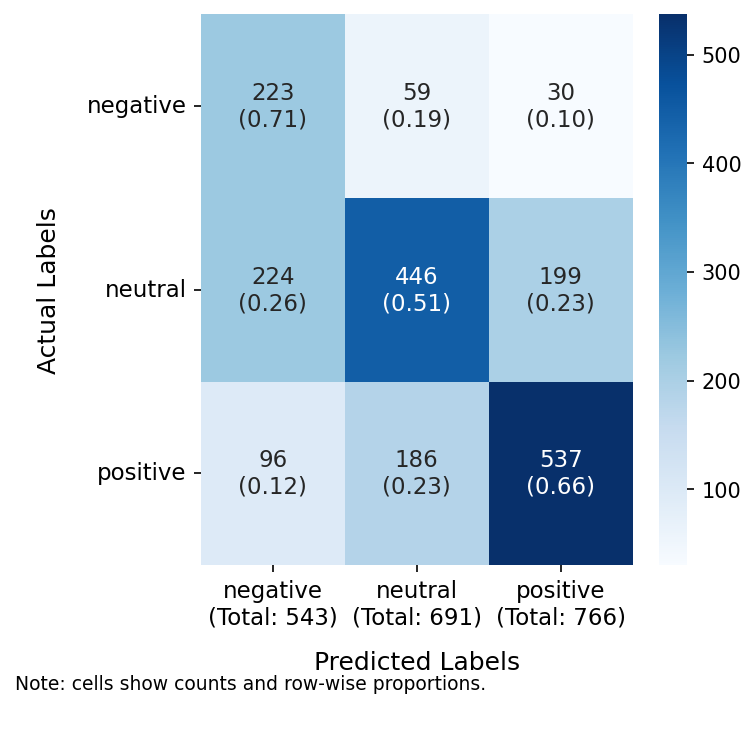
\includegraphics[width=0.7\textwidth]{media/cm_run1_embeddings_LR.png}
\caption{Confusion matrix: 3-class logistic regression with embeddings (macro F1 = 0.590). Errors spread realistically across all three classes --- the model is uncertain, not just defaulting to neutral.}
\label{fig:cm_lr_embeddings}
\end{figure}



\subsection*{4.3 RUN 2: 3-class classification, decision tree}



The decision tree performed substantially worse than logistic regression across most feature configurations. With unigram features and max\_depth=3, its macro F1 was 0.277---barely above the 0.333 floor of random chance. It predominantly predicts neutral for most inputs.

But it's not just weaker---it fails in a totally different way. Logistic regression spreads its mistakes around. The tree just gives up and uses a trivial heuristic. Three levels deep isn't enough for anything subtle.

Accuracy for the tree? 0.474. Logistic regression? 0.470. Practically the same. But this is exactly why accuracy is the wrong metric for imbalanced multi-class problems. Macro F1 catches this; accuracy hides it. Running both models side by side on this dataset taught me more than any textbook example. Figure~\ref{fig:cm_dt_unigrams} shows the extent of this collapse.

\begin{figure}[h]
\centering
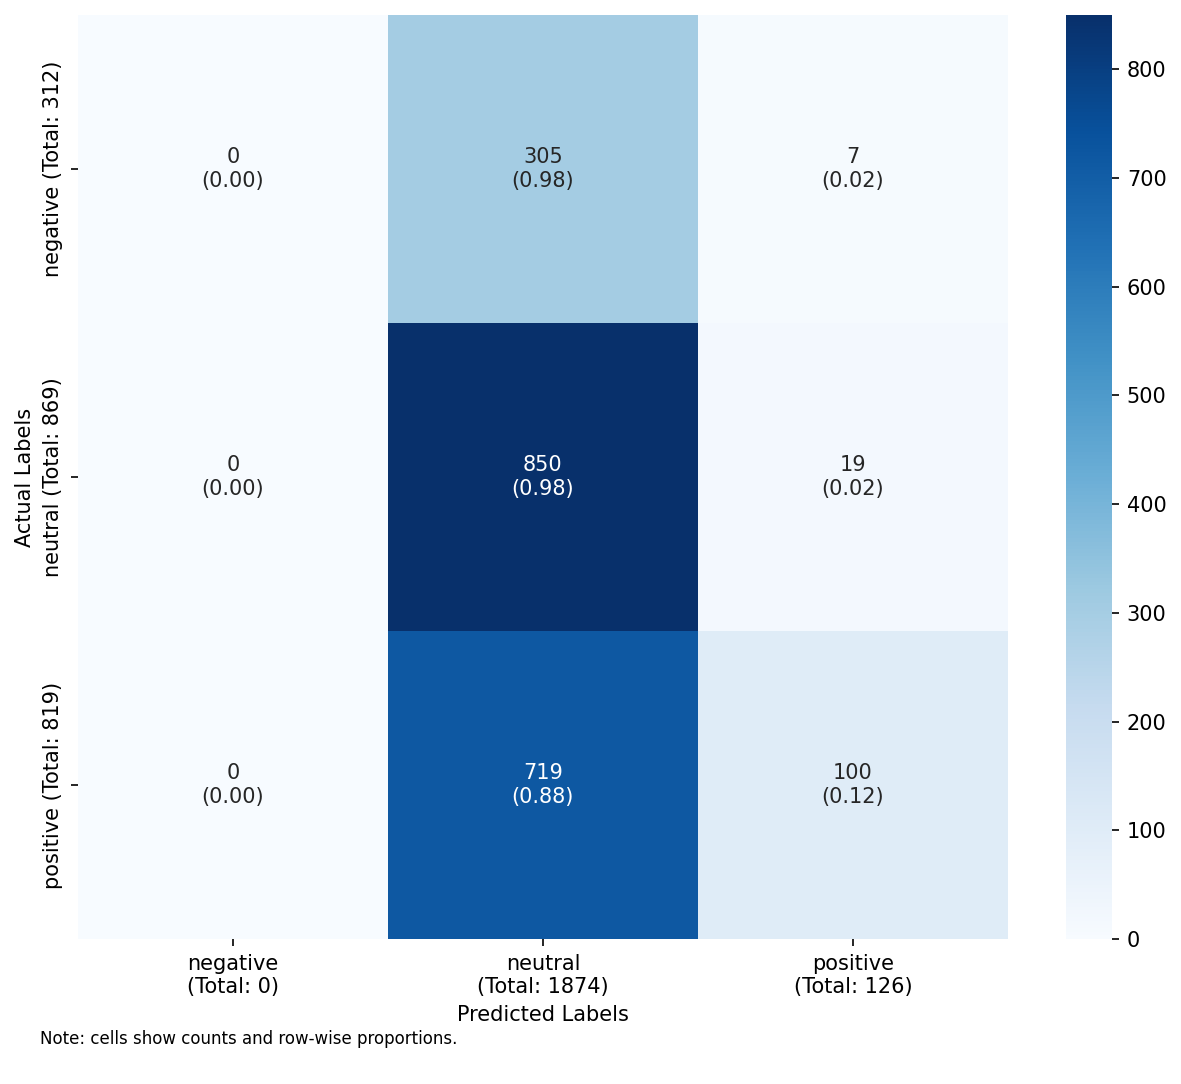
\includegraphics[width=0.7\textwidth]{media/cm_run2_unigrams_DT.png}
\caption{Confusion matrix: 3-class decision tree with unigrams (macro F1 = 0.277). The tree predicts neutral for almost every input --- recall for negative and positive is near zero.}
\label{fig:cm_dt_unigrams}
\end{figure}



\subsection*{4.4 3-class vs binary: gain summary}



\begin{table}[h]
\centering
\caption{Macro F1 for 3-class and binary tasks, and gain from removing neutral.}
\label{tab:gain}
\small
\begin{tabular}{lrrr@{\hspace{2em}}rrr}
\toprule
& \multicolumn{3}{c}{Logistic Regression} & \multicolumn{3}{c}{Decision Tree} \\
\cmidrule(lr){2-4} \cmidrule(lr){5-7}
Feature set & 3-class & binary & gain & 3-class & binary & gain \\
\midrule
unigrams   & 0.466 & 0.667 & +0.201 & 0.277 & 0.521 & +0.244 \\
bigrams    & 0.335 & 0.525 & +0.190 & 0.232 & 0.448 & +0.217 \\
uni+pos    & 0.472 & 0.650 & +0.178 & 0.327 & 0.561 & +0.234 \\
textstats  & 0.387 & 0.540 & +0.154 & 0.369 & 0.553 & +0.184 \\
lexicon    & 0.540 & 0.639 & +0.099 & 0.539 & 0.638 & +0.098 \\
embeddings & 0.590 & 0.806 & +0.216 & 0.419 & 0.614 & +0.195 \\
\bottomrule
\end{tabular}
\end{table}



\section*{5 Discussion}



\subsection*{5.1 Overall performance}



The logistic regression baseline achieved a macro F1 of 0.447 on the 3-class task.
A score below 0.5 is not strong, but it is not meaningless.
With the level of annotation noise present and the known difficulty of the neutral class, a macro F1 in the 0.4--0.5 range is a credible baseline.
A random classifier on a balanced three-class problem would achieve macro F1 of 0.333.
So 0.447 from logistic regression is comfortably above both floors.

The decision tree's macro F1 was 0.277.
Accuracy? 0.474, basically the same as logistic regression (0.470).
With 43.5\% neutral in the test set, a model can just say ``neutral'' for every input and score 43.5\% accuracy without learning anything.
Macro F1 exposes this; accuracy conceals it.



\subsection*{5.2 Feature comparison}



The six feature configurations produced different results, and a few patterns stood out.
VADER I felt better about --- it was designed for social media, encodes human judgements about sentiment, and incorporates slang and emoticons that general vocabulary counts miss.
\citet{hutto2014vader} showed it worked well on Twitter data, and this task felt very close to what they evaluated it on.
Embeddings I was less certain about going in.
If they came from generic text rather than social media, I expected they'd struggle with informal shorthand like ``can't even rn''.

One pattern I noticed when comparing feature configurations: the per-class ordering remains stable.
In logistic regression, per-class F1 almost always follows negative $<$ positive $<$ neutral, even as the absolute values vary.
I believe this suggests the relative difficulty of each class is a property of the data rather than any particular feature representation.
The negative class is harder to classify regardless of the features used---that is a data observation, not a modelling one.



\subsection*{5.3 What the binary task reveals}



Sub-question 4 is really asking: was neutral the problem all along, or is the trouble more general?

Table~\ref{tab:gain} shows macro F1 for both setups and the gain from dropping neutral.
Big, consistent gains would suggest neutral is mostly to blame.
Small or variable gains would suggest the problem is spread more evenly.



\subsection*{5.4 Class-level analysis}



The 3-class LR results are not balanced across classes.
Positive tweets got the best F1, with high precision but only middling recall.
Negative is the worst performer: low precision, moderate recall.
Neutral sits in the middle.

I didn't expect neutral to beat negative, but it did.
The conventional view---supported by \citet{kenyondean2018sentiment}---is that neutral is the hardest class because it lacks distinctive lexical markers.
The results don't clearly support this.
Maybe that's because neutral is the largest group in the test set, giving the model more evaluation signal.
Or maybe neutral tweets cluster around non-sentiment-loaded vocabulary that shows up well in the top-200 unigrams.

The decision tree collapse is a separate phenomenon.
It's not just weak on negative and positive---it's nearly zero on both.
The tree has apparently learned that predicting neutral minimises loss on the training data even after undersampling.
That bothers me.
It suggests the feature representations don't yield a clean split between neutral and the other classes at any single threshold.



\subsection*{5.5 Label quality evidence}



The thing I kept returning to is that a low macro F1 doesn't tell you much on its own.
It could be the features, the model, the labels, or all three.
All three are probably true to some degree here, and I genuinely cannot tell which dominates.

Negative stands out. Low precision means the model generates many false positive predictions for negative sentiment. If the model predicts negative based on reasonable lexical cues but the gold label is neutral, this suggests annotators labelled borderline tweets as neutral rather than negative. The neutral label may have introduced systematic ambiguity in this dataset \citep{kenyondean2018sentiment}:

\begin{itemize}

  \item the category was designed to capture genuine neutrality alongside mild negative expression;

  \item annotators were uncertain about tweets that fell between the two;

  \item sentiment is a property of the author's relationship to content, not just of the words used.

\end{itemize}

A phrase like ``not bad at all'' could be positive or ironic depending on context. Unigram count features are poorly equipped to capture these distinctions. Even human annotators would disagree on these cases; the low classifier performance may be tracking that annotator disagreement rather than merely reflecting model inadequacy.



\subsection*{5.6 Misclassification analysis}



I ran the misclassification breakdown in notebook section 4.2.
Some misclassifications are model failures.
Other misclassifications are more interesting. When I checked tweets the model called negative but the label was neutral, a recurring pattern came up:

\begin{itemize}

  \item tweets expressing mild dissatisfaction, slight frustration, or low-key complaint;

  \item the kind of expression that sits at the boundary between neutral and negative in everyday language.

\end{itemize} I'd expect human annotators to disagree on these. The model isn't clearly wrong. The label isn't clearly right. That ambiguity is the point.

Across all feature configurations, the tweets the model consistently misses are the sarcastic, ironic, or context-dependent ones. No unigram or bigram feature set can resolve this. That's a hard ceiling for surface-form features, and it's a real constraint.



\subsection*{5.7 Limitations and future directions}



There are things I couldn't do, or wish I'd done differently.

I set max\_depth=3 deliberately --- I wanted to see the actual splits, not just get the highest score.
A deeper tree would likely do better on F1, but I'd lose the ability to read it.

The embeddings used here are from a pre-trained general-purpose model. Fine-tuning on Twitter data would likely produce more useful tweet embeddings. General models just don't always capture the quirks of short text.

The analysis is constrained to the validation split. The held-out test split (12,284 tweets) has not been used and would provide a more reliable estimate of generalisation performance. The validation set has only 312 negative examples, which limits the precision of per-class estimates for that class.

The labels themselves are uncertain in ways I can't fix. They're majority-vote outcomes, not ground truth. Without inter-annotator agreement scores, I cannot distinguish ``model failure'' from ``contested annotation.'' That is probably the most valuable extension of this analysis.



\nocite{*}

\bibliographystyle{apalike}

\bibliography{refs}

\appendix

\section{How to Run the Submission Package}

The notebook can be run manually in the usual way, but I've spent some time automating this.
The main reason is that the notebook uses relative paths and creates sibling folders during execution --- so where you open it matters.
Here is what I'd recommend.

This submission is distributed as a zip archive.
When unpacking, keep the top-level folder \texttt{FINAL-PROJECT/} intact.
Open the notebook from inside \texttt{FINAL-PROJECT/python/} --- do not move it elsewhere.

For one-line execution after extraction, run \texttt{python run\_submission.py} from the package root.
This launcher executes the notebook via Jupyter \texttt{nbconvert}.

This is important because the notebook uses relative paths and expects enough headroom under \texttt{FINAL-PROJECT/} to create and use sibling folders such as \texttt{data/}, \texttt{figs/}, \texttt{results/}, and \texttt{report/}.
If the folder structure is preserved, no extra setup instructions should be needed by the user.
After the first run has created these working folders, the notebook can also be run manually in the usual way, provided it remains in the same \texttt{FINAL-PROJECT/python/} location.

\begin{verbatim}
  python -m zipfile -e FINAL-PROJECT-SUBMISSION.zip .
  python run_submission.py
\end{verbatim}

\section{All Confusion Matrices}

The figures below show confusion matrices for every feature configuration across all four runs.
RUN 1 and RUN 2 are 3-class (negative, neutral, positive); RUN 3 and RUN 4 are binary (negative vs positive).
Each matrix is normalised by true label so the diagonal shows recall per class.

\subsection*{RUN 1 --- 3-class, Logistic Regression}

\begin{figure}[ht]
  \centering
  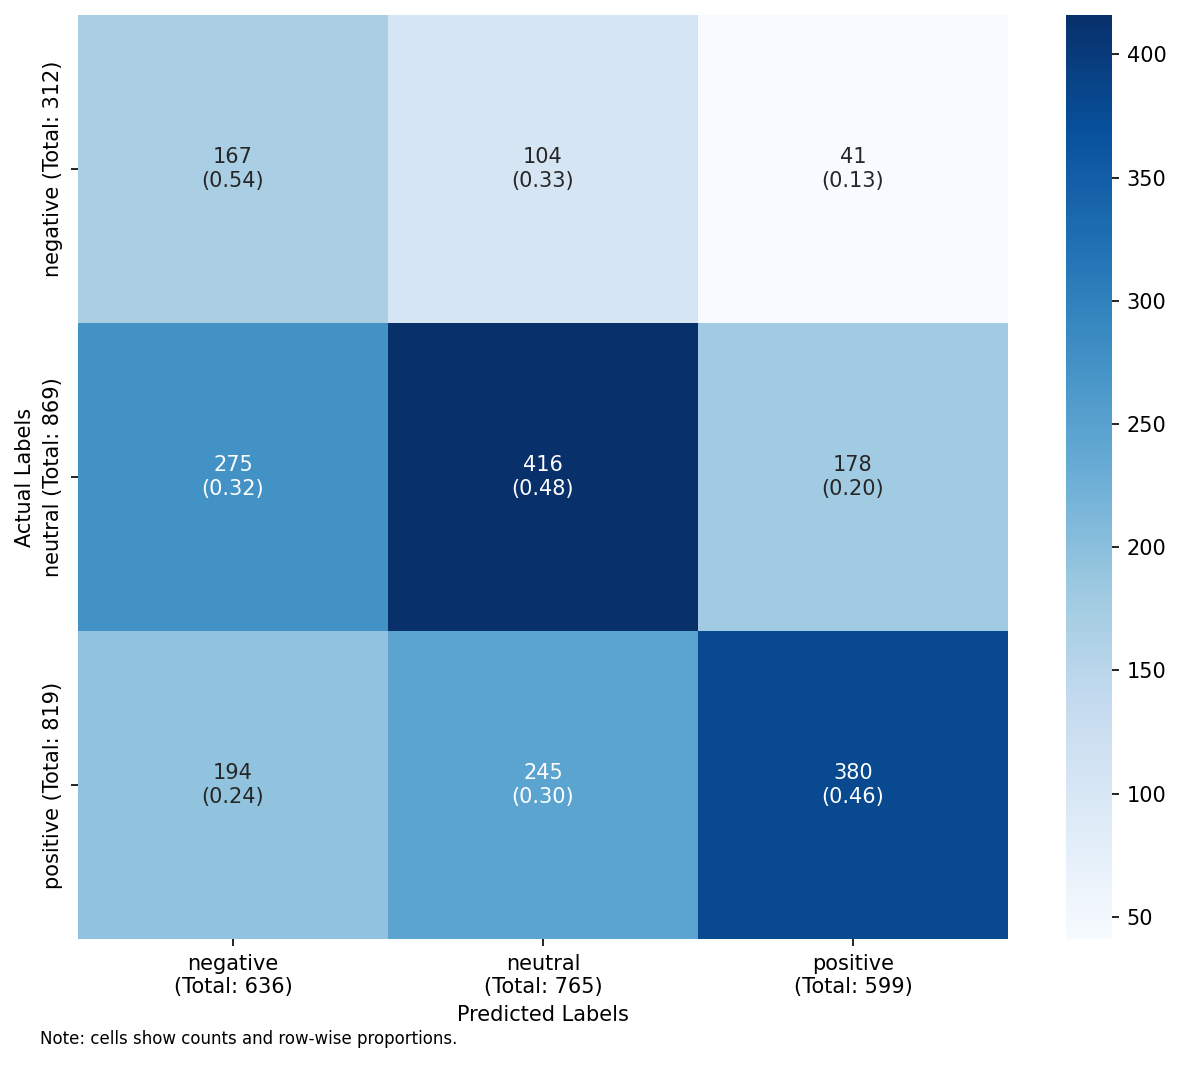
\includegraphics[width=0.48\textwidth]{media/cm_run1_unigrams_LR.png}
  \hfill
  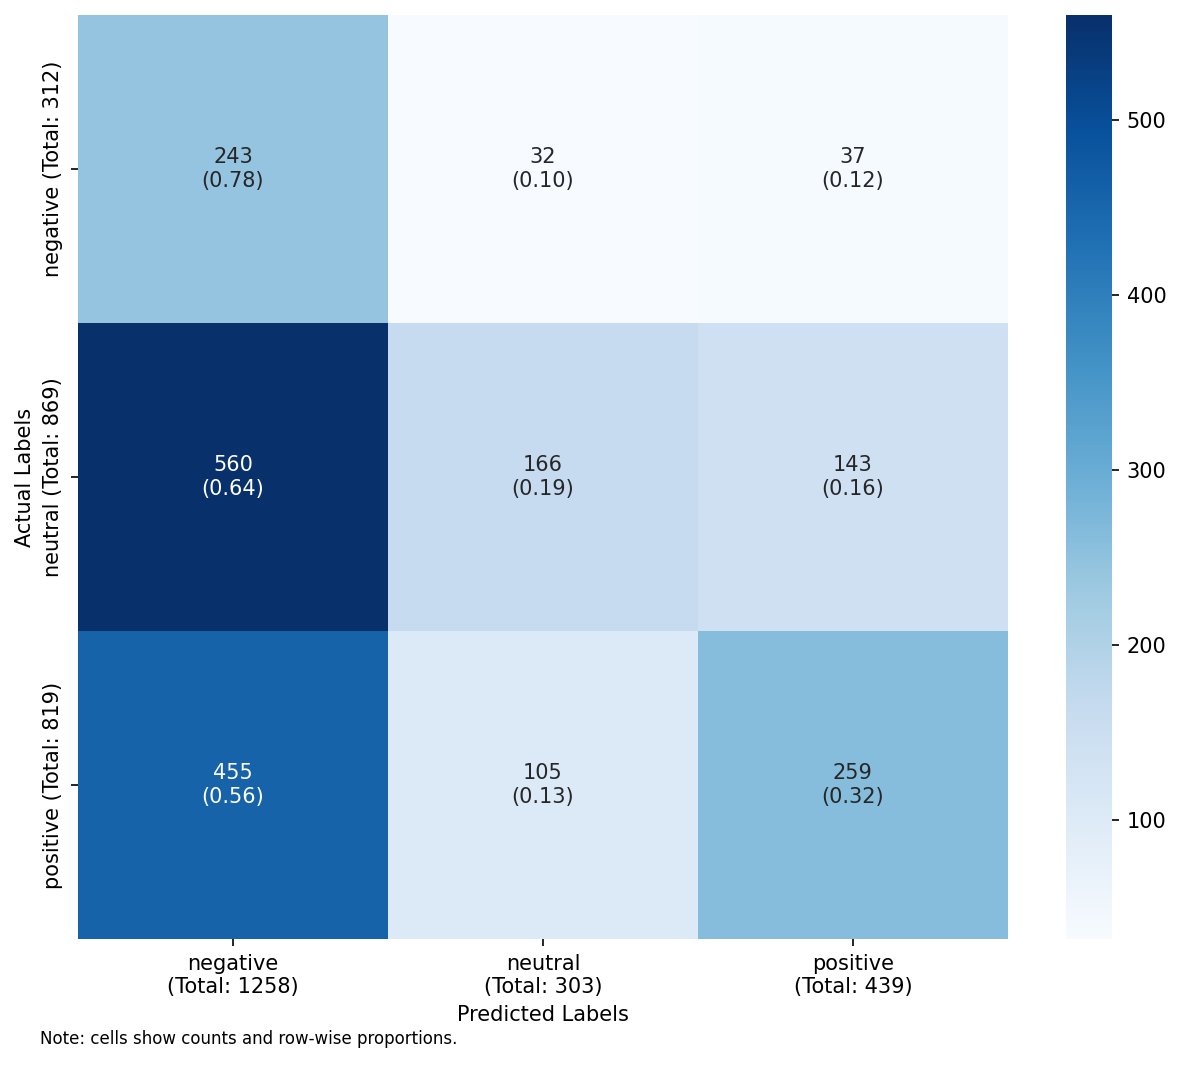
\includegraphics[width=0.48\textwidth]{media/cm_run1_bigrams_LR.png}
  \caption{RUN 1 LR: unigrams (left), bigrams (right)}
\end{figure}

\begin{figure}[ht]
  \centering
  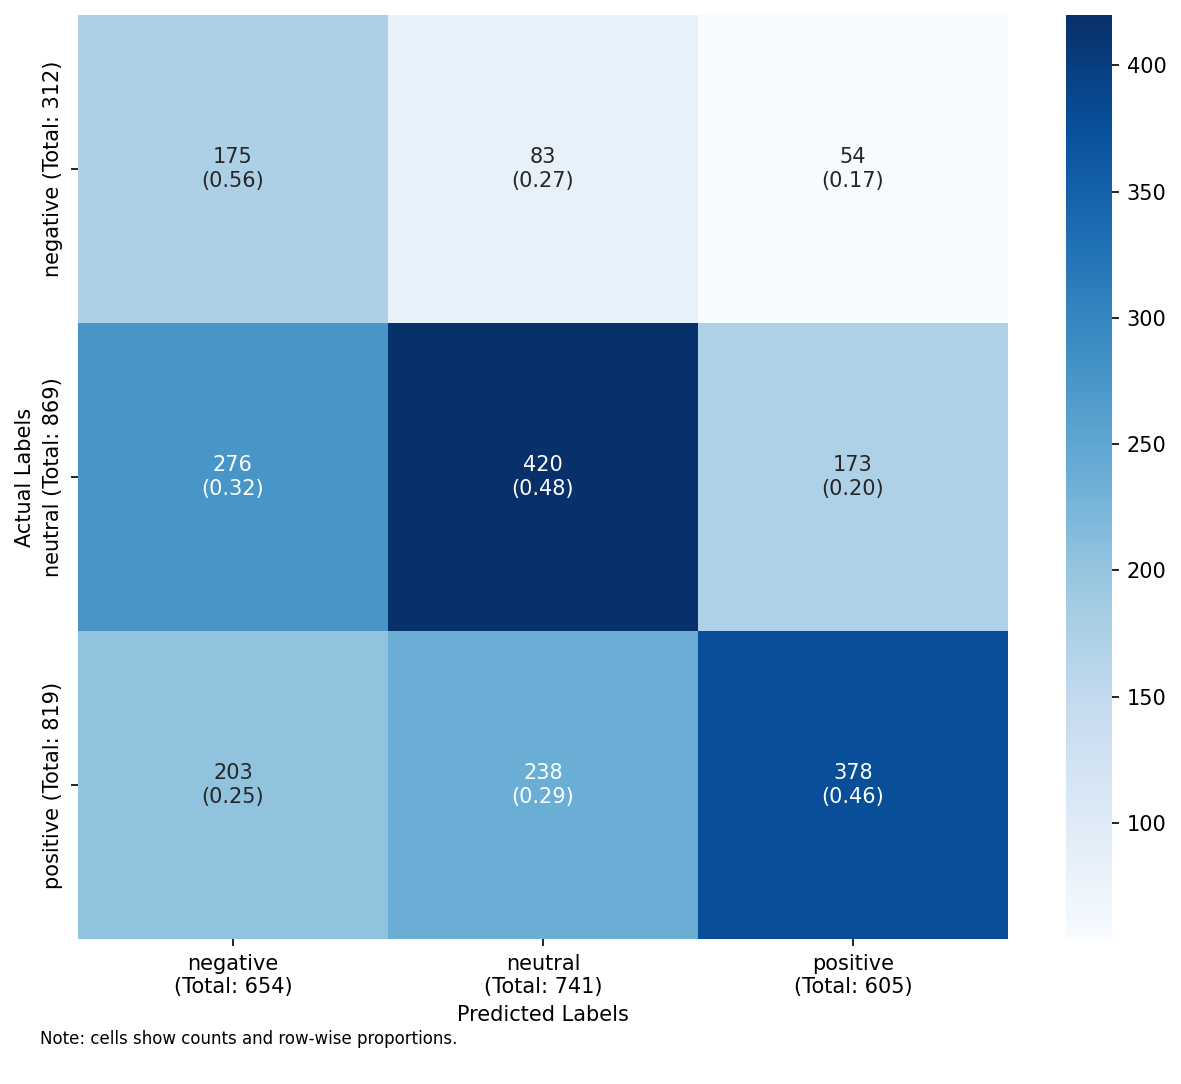
\includegraphics[width=0.48\textwidth]{media/cm_run1_uni+pos_LR.png}
  \hfill
  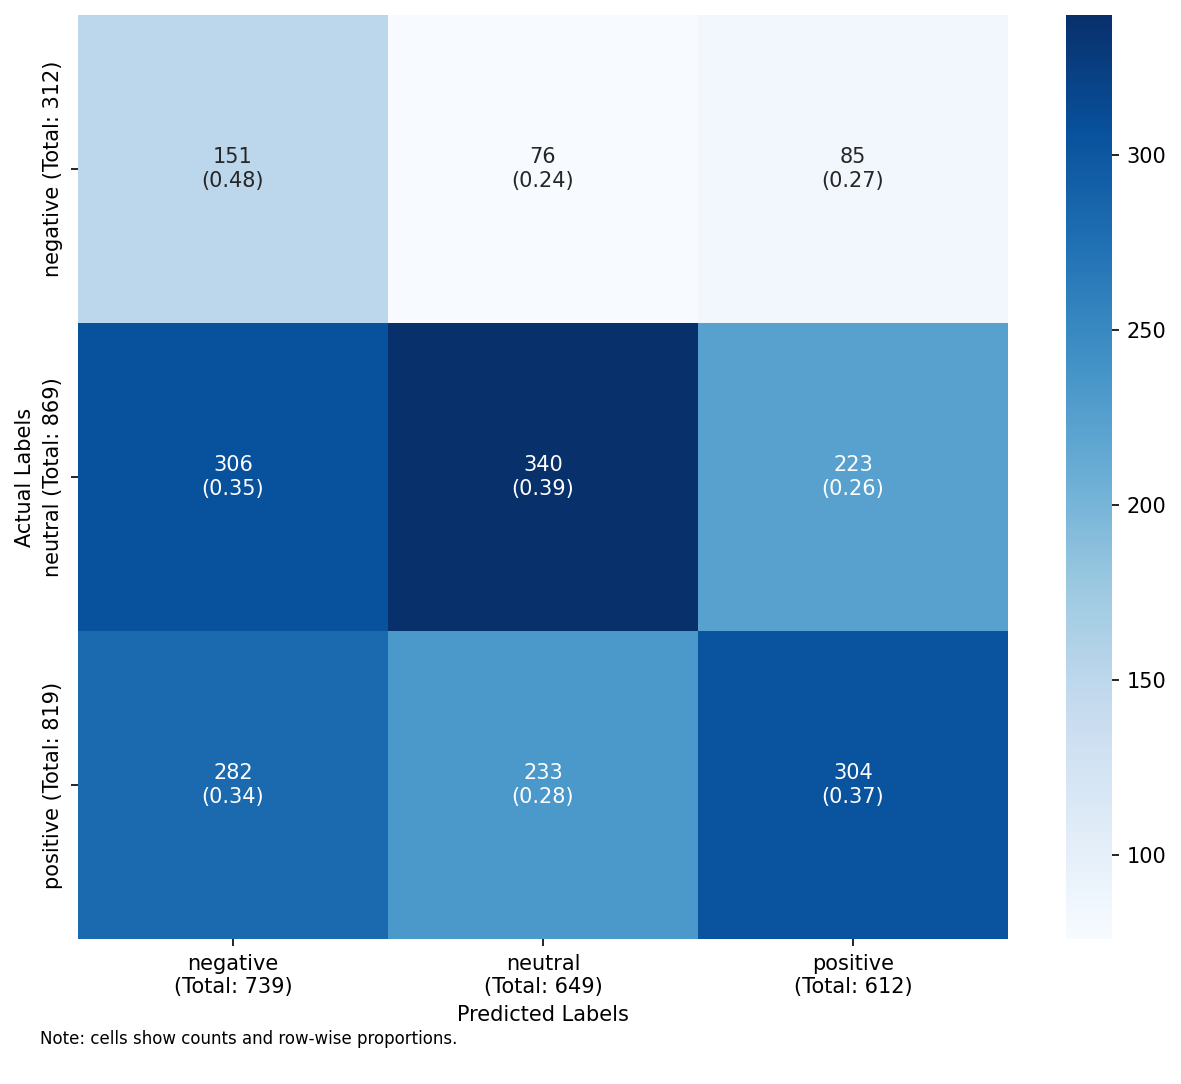
\includegraphics[width=0.48\textwidth]{media/cm_run1_textstats_LR.png}
  \caption{RUN 1 LR: unigrams+POS (left), text statistics (right)}
\end{figure}

\begin{figure}[ht]
  \centering
  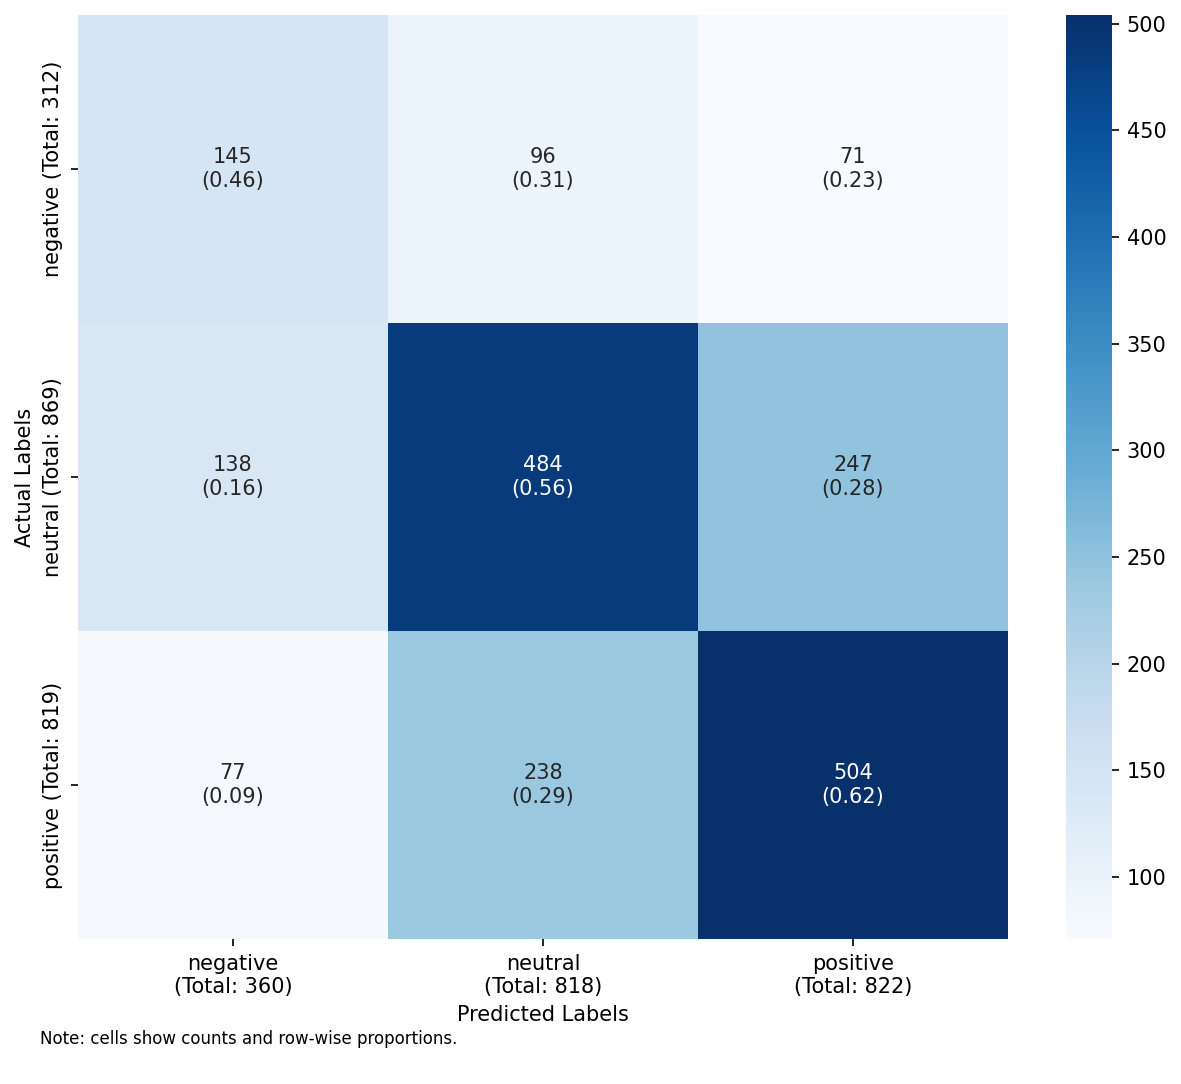
\includegraphics[width=0.48\textwidth]{media/cm_run1_lexicon_LR.png}
  \hfill
  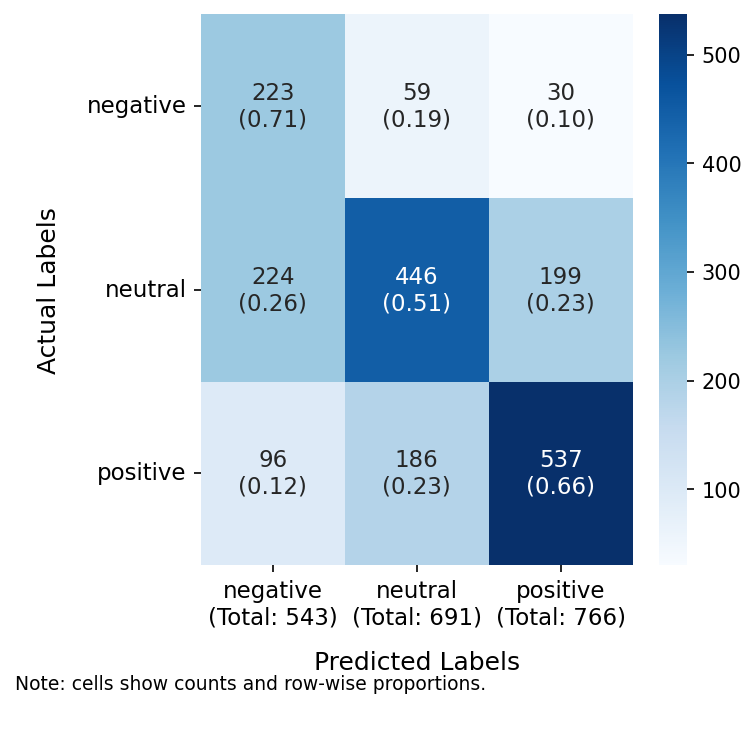
\includegraphics[width=0.48\textwidth]{media/cm_run1_embeddings_LR.png}
  \caption{RUN 1 LR: lexicon (left), embeddings (right)}
\end{figure}

\subsection*{RUN 2 --- 3-class, Decision Tree}

\begin{figure}[ht]
  \centering
  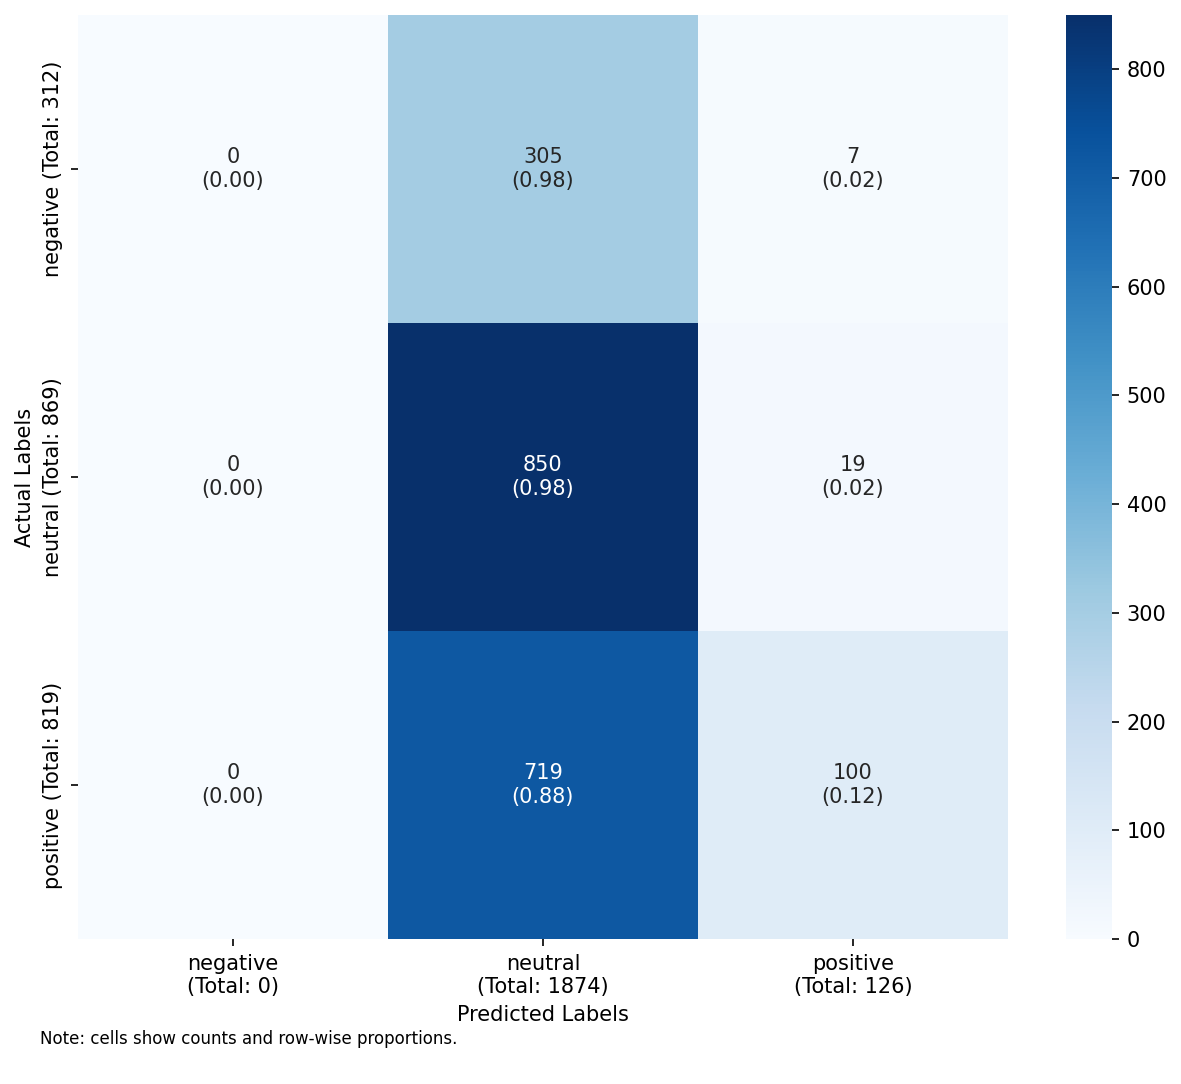
\includegraphics[width=0.48\textwidth]{media/cm_run2_unigrams_DT.png}
  \hfill
  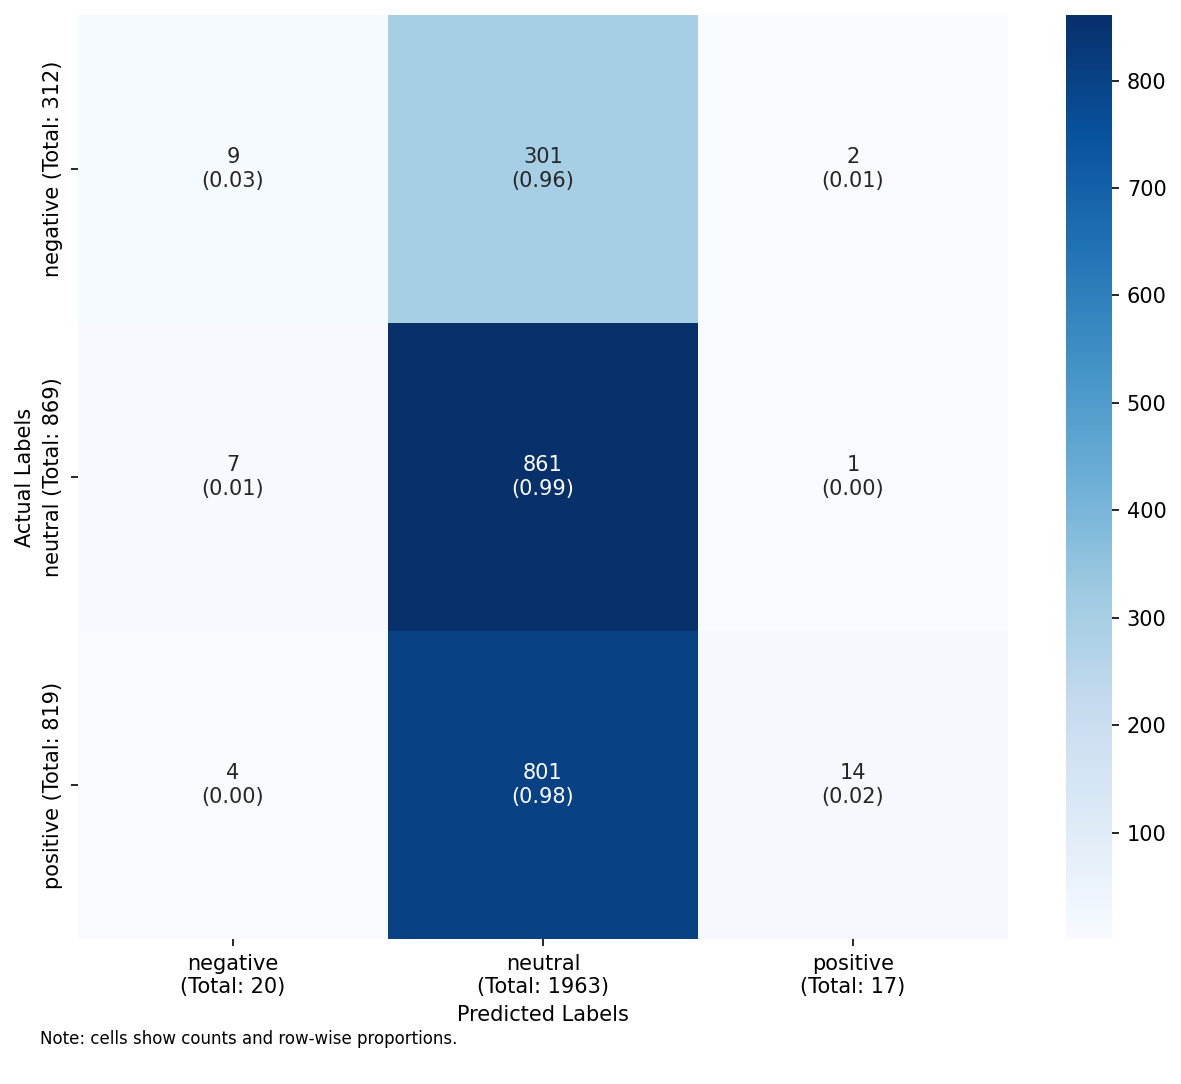
\includegraphics[width=0.48\textwidth]{media/cm_run2_bigrams_DT.png}
  \caption{RUN 2 DT: unigrams (left), bigrams (right)}
\end{figure}

\begin{figure}[ht]
  \centering
  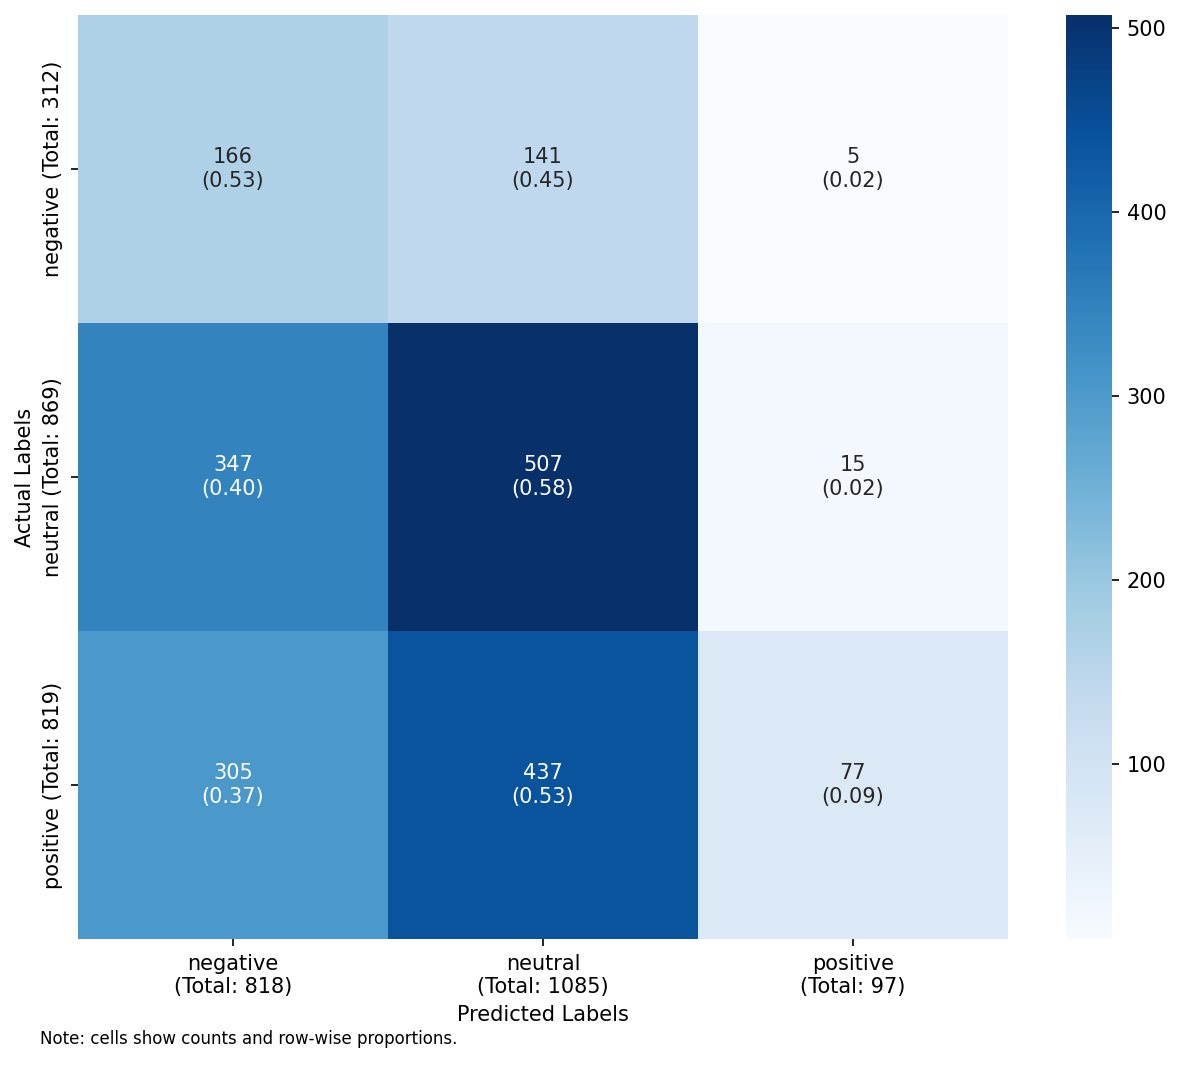
\includegraphics[width=0.48\textwidth]{media/cm_run2_uni+pos_DT.png}
  \hfill
  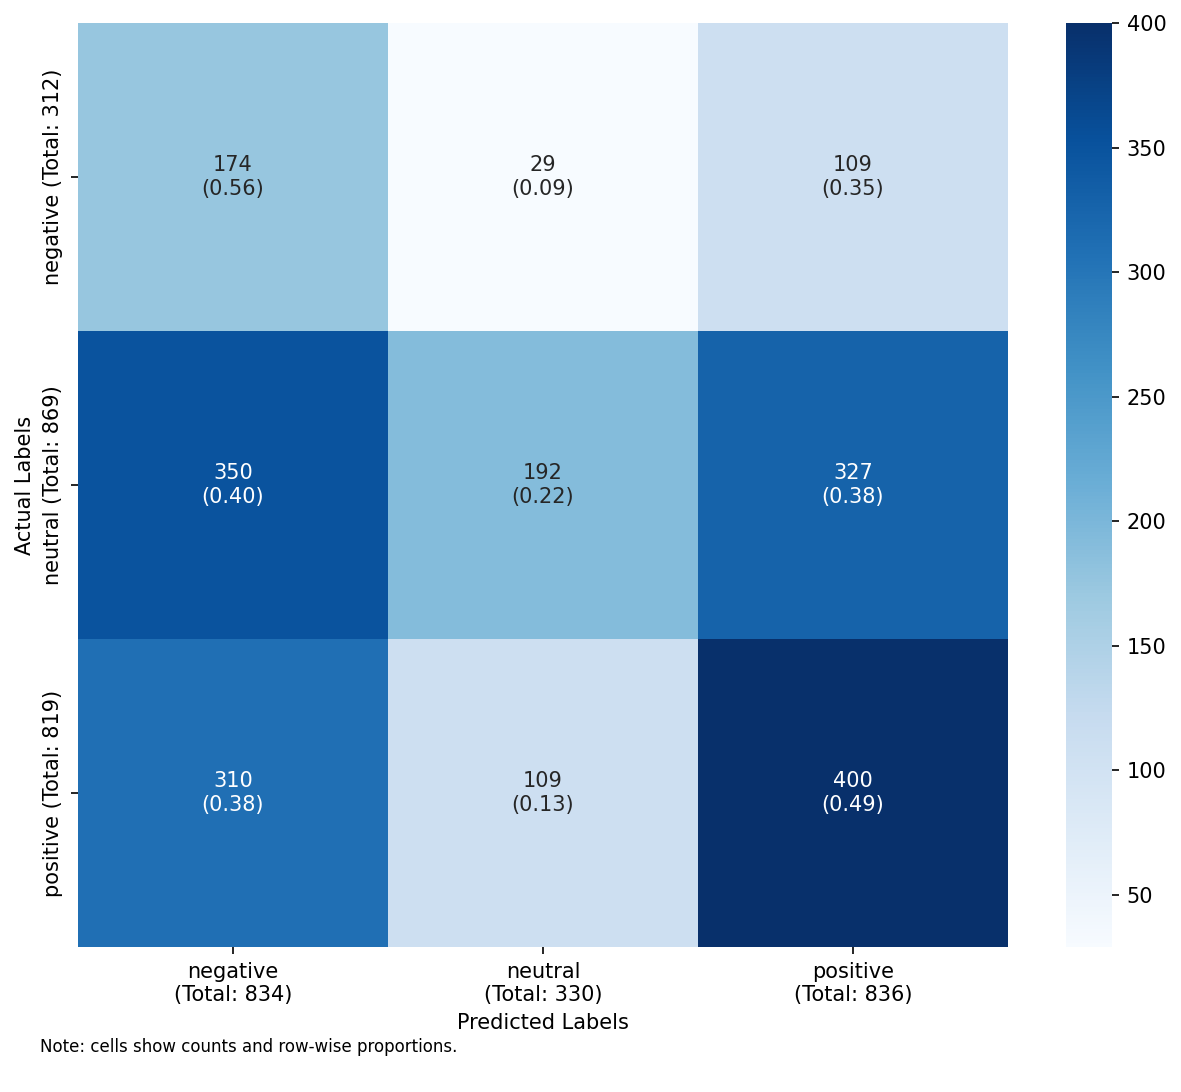
\includegraphics[width=0.48\textwidth]{media/cm_run2_textstats_DT.png}
  \caption{RUN 2 DT: unigrams+POS (left), text statistics (right)}
\end{figure}

\begin{figure}[ht]
  \centering
  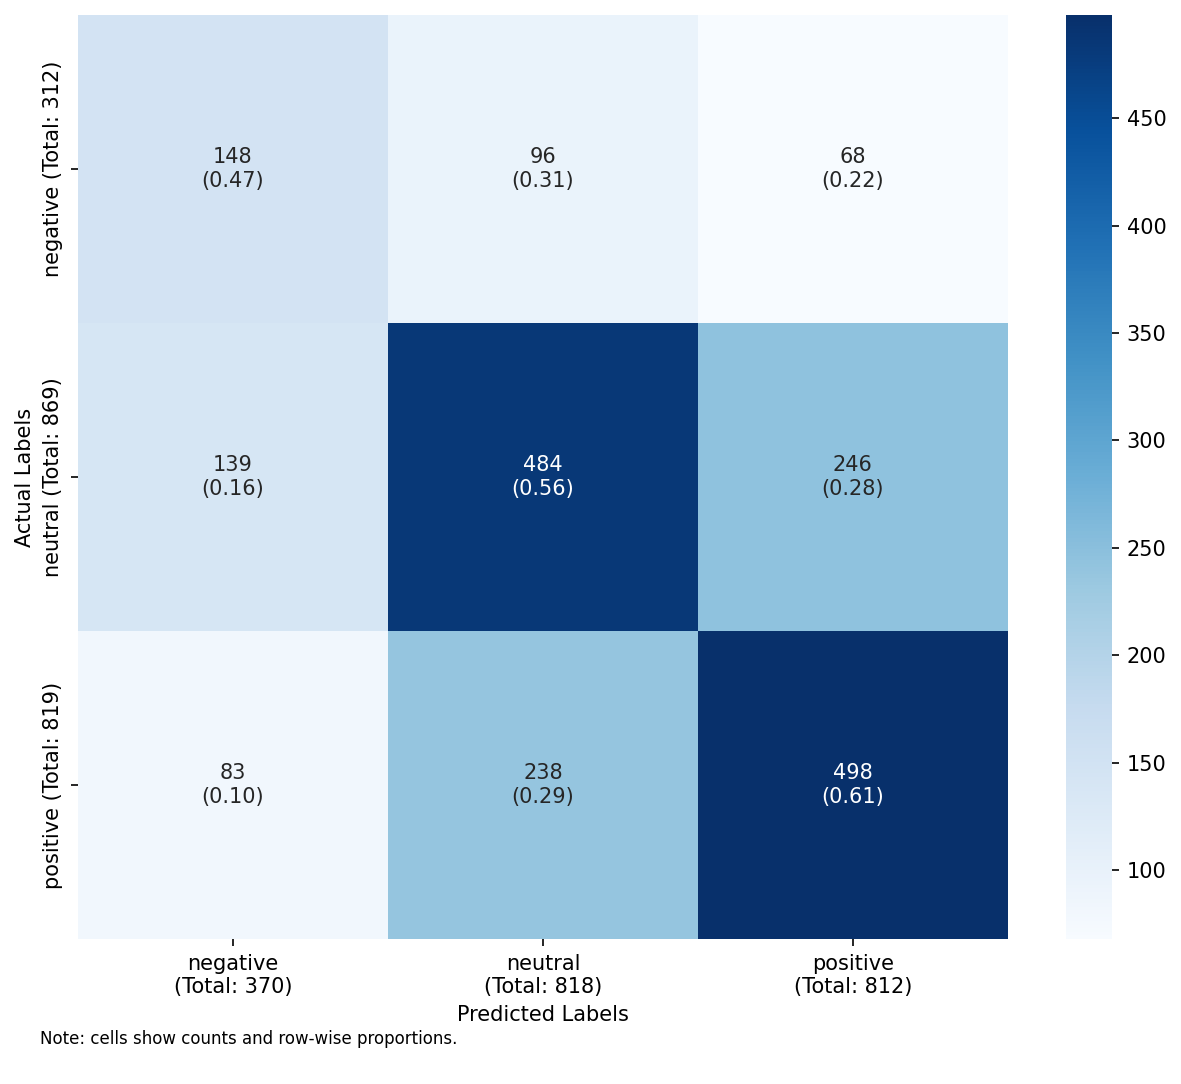
\includegraphics[width=0.48\textwidth]{media/cm_run2_lexicon_DT.png}
  \hfill
  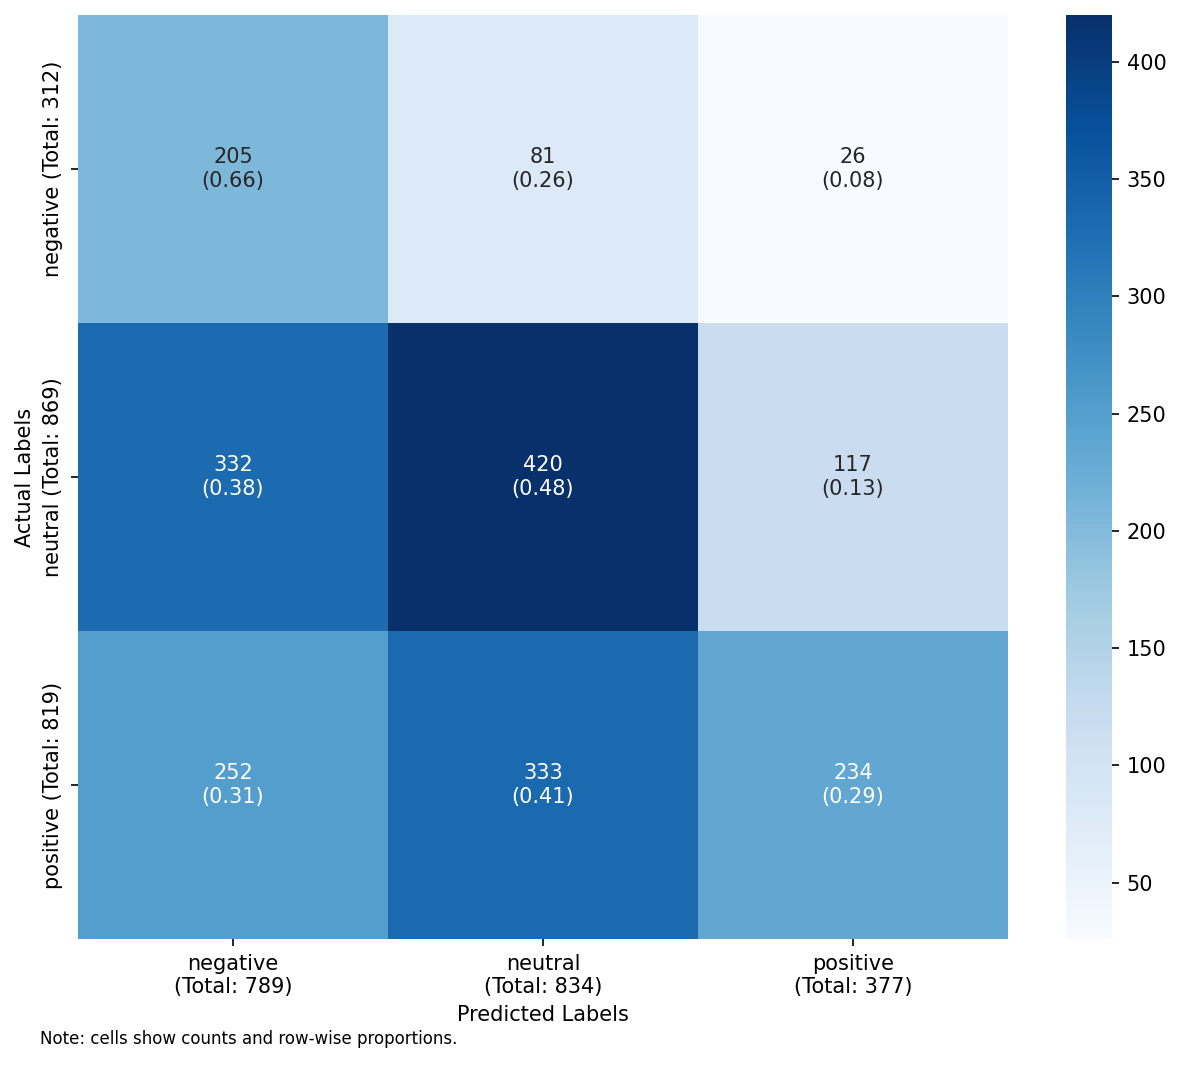
\includegraphics[width=0.48\textwidth]{media/cm_run2_embeddings_DT.png}
  \caption{RUN 2 DT: lexicon (left), embeddings (right)}
\end{figure}

\subsection*{RUN 3 --- binary, Logistic Regression}

\begin{figure}[ht]
  \centering
  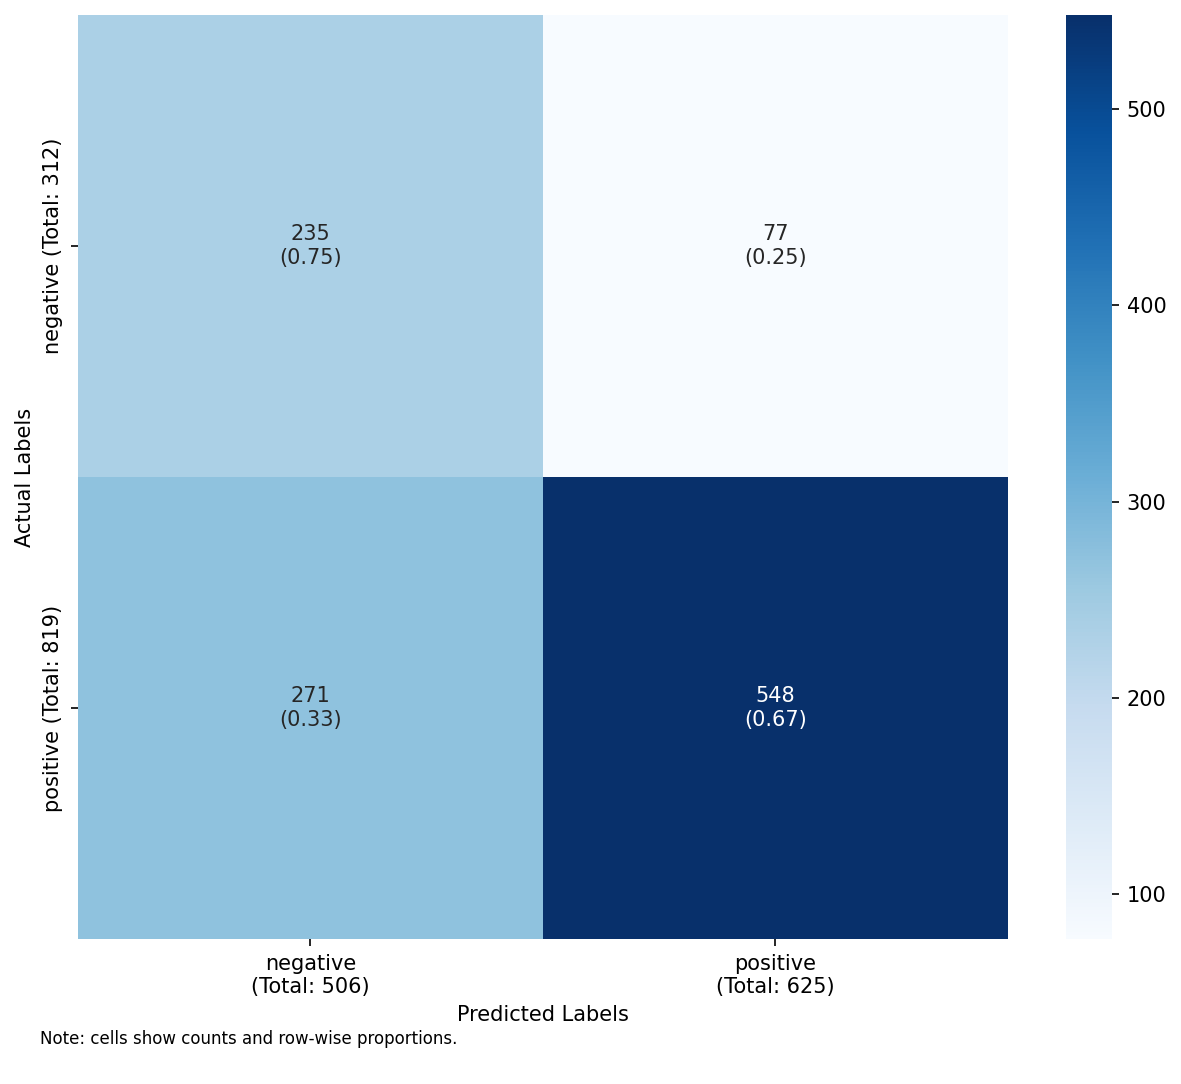
\includegraphics[width=0.48\textwidth]{media/cm_run3_unigrams_LR.png}
  \hfill
  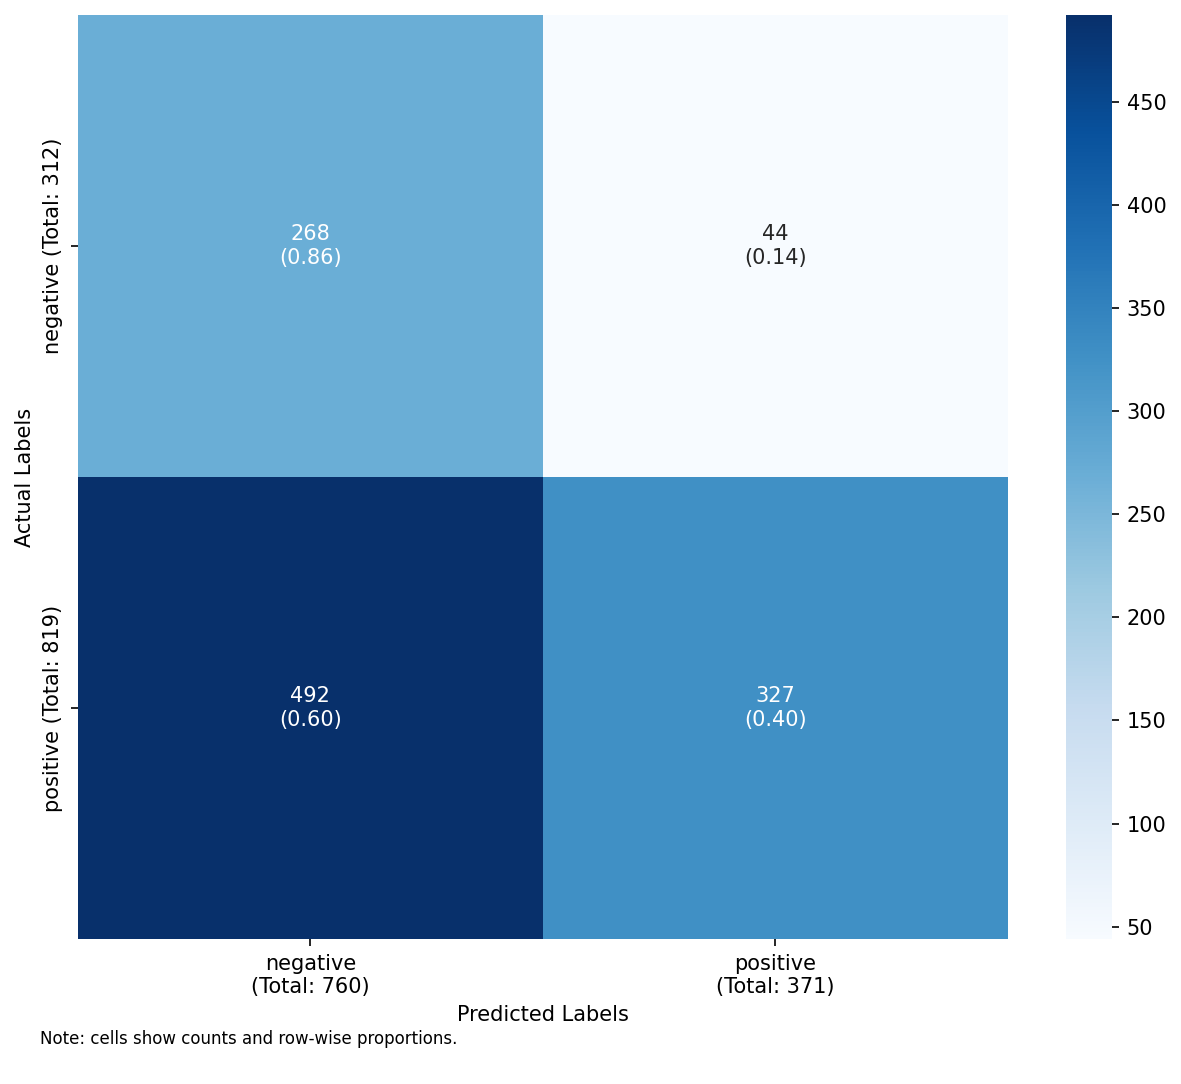
\includegraphics[width=0.48\textwidth]{media/cm_run3_bigrams_LR.png}
  \caption{RUN 3 LR: unigrams (left), bigrams (right)}
\end{figure}

\begin{figure}[ht]
  \centering
  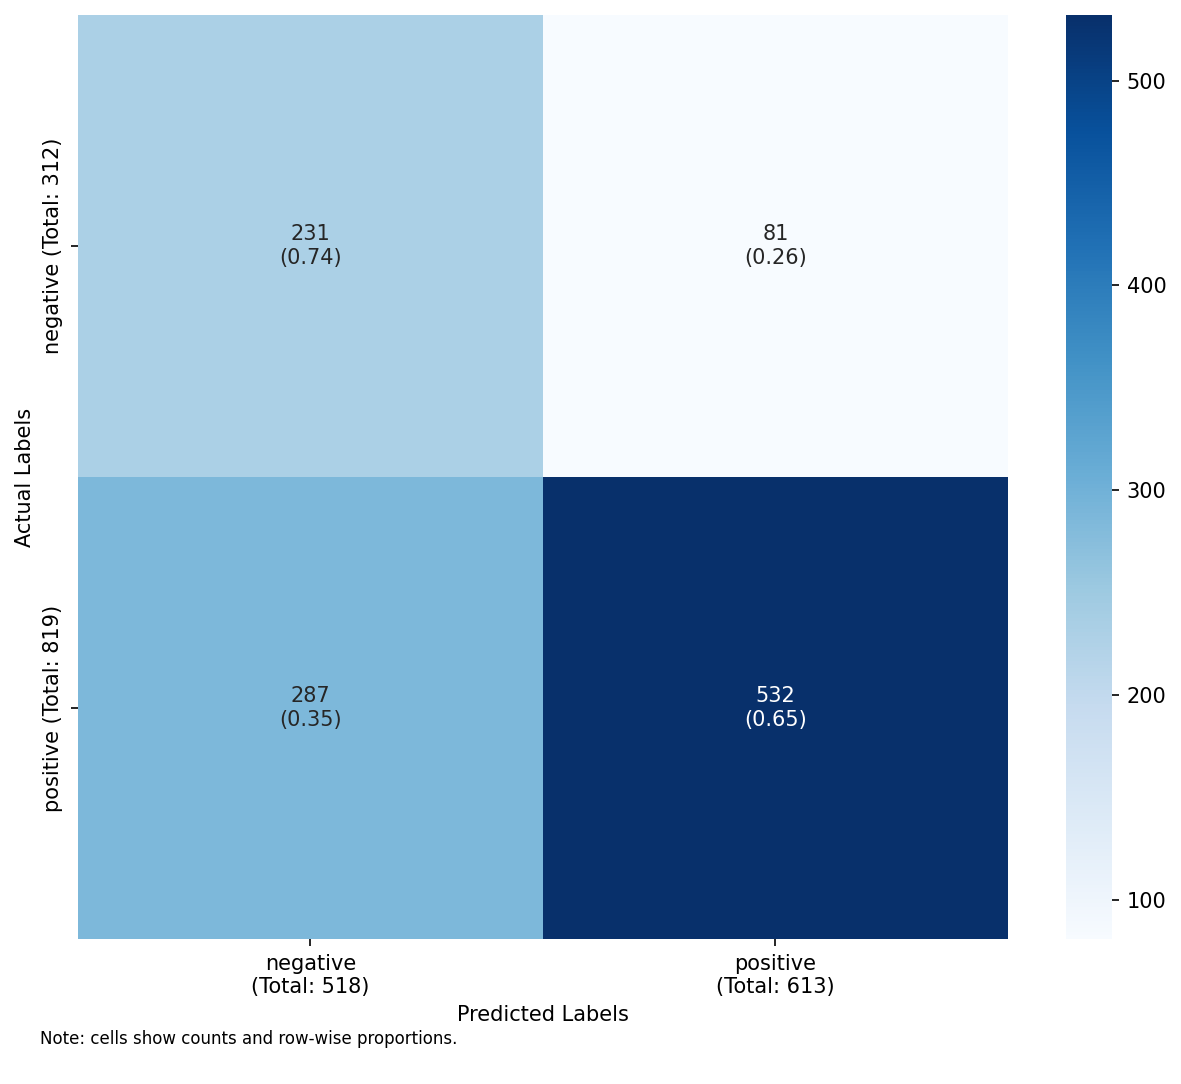
\includegraphics[width=0.48\textwidth]{media/cm_run3_uni+pos_LR.png}
  \hfill
  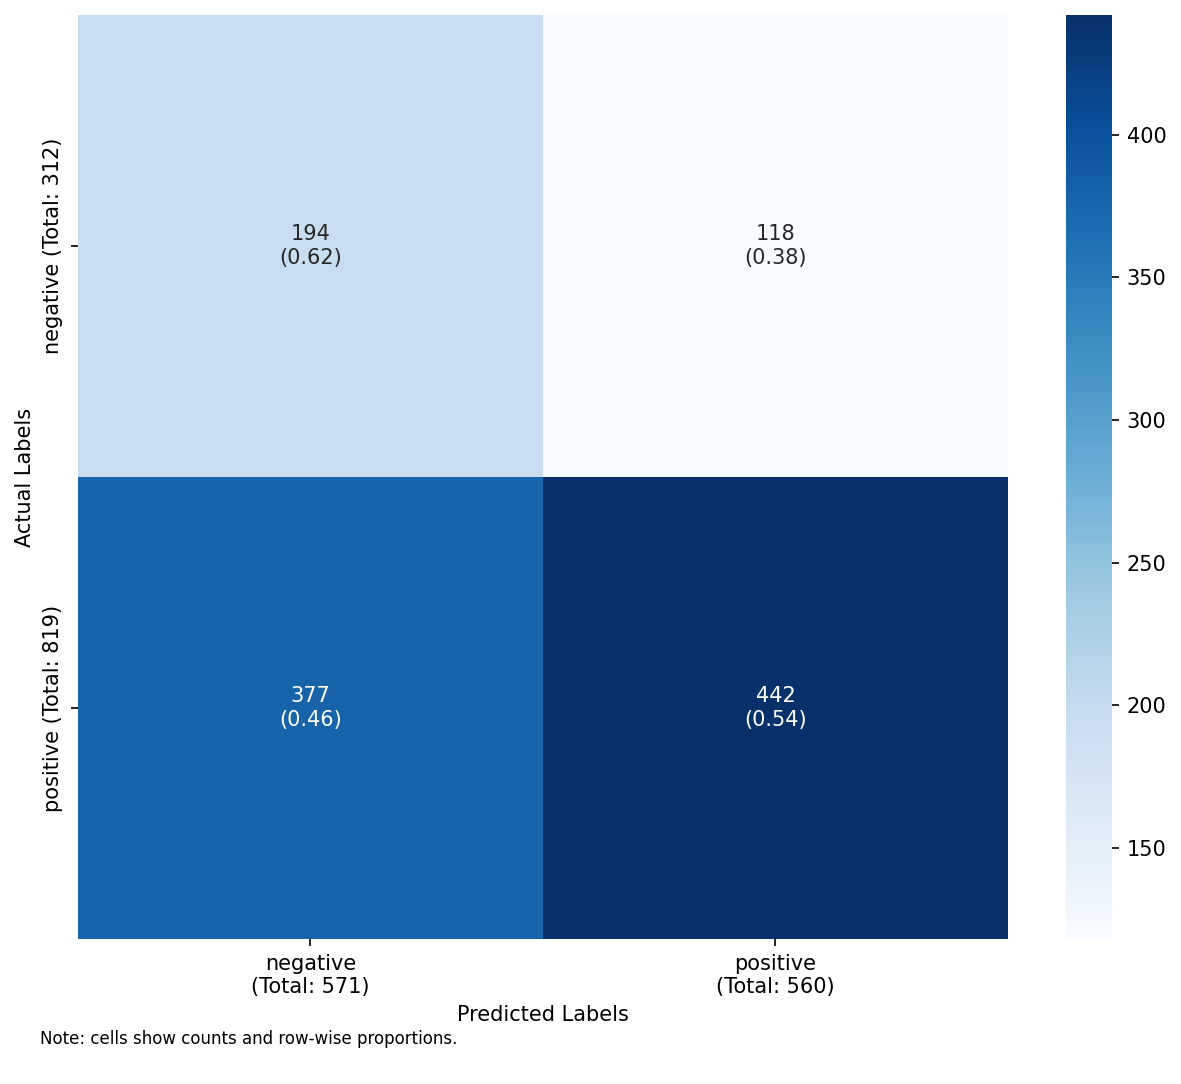
\includegraphics[width=0.48\textwidth]{media/cm_run3_textstats_LR.png}
  \caption{RUN 3 LR: unigrams+POS (left), text statistics (right)}
\end{figure}

\begin{figure}[ht]
  \centering
  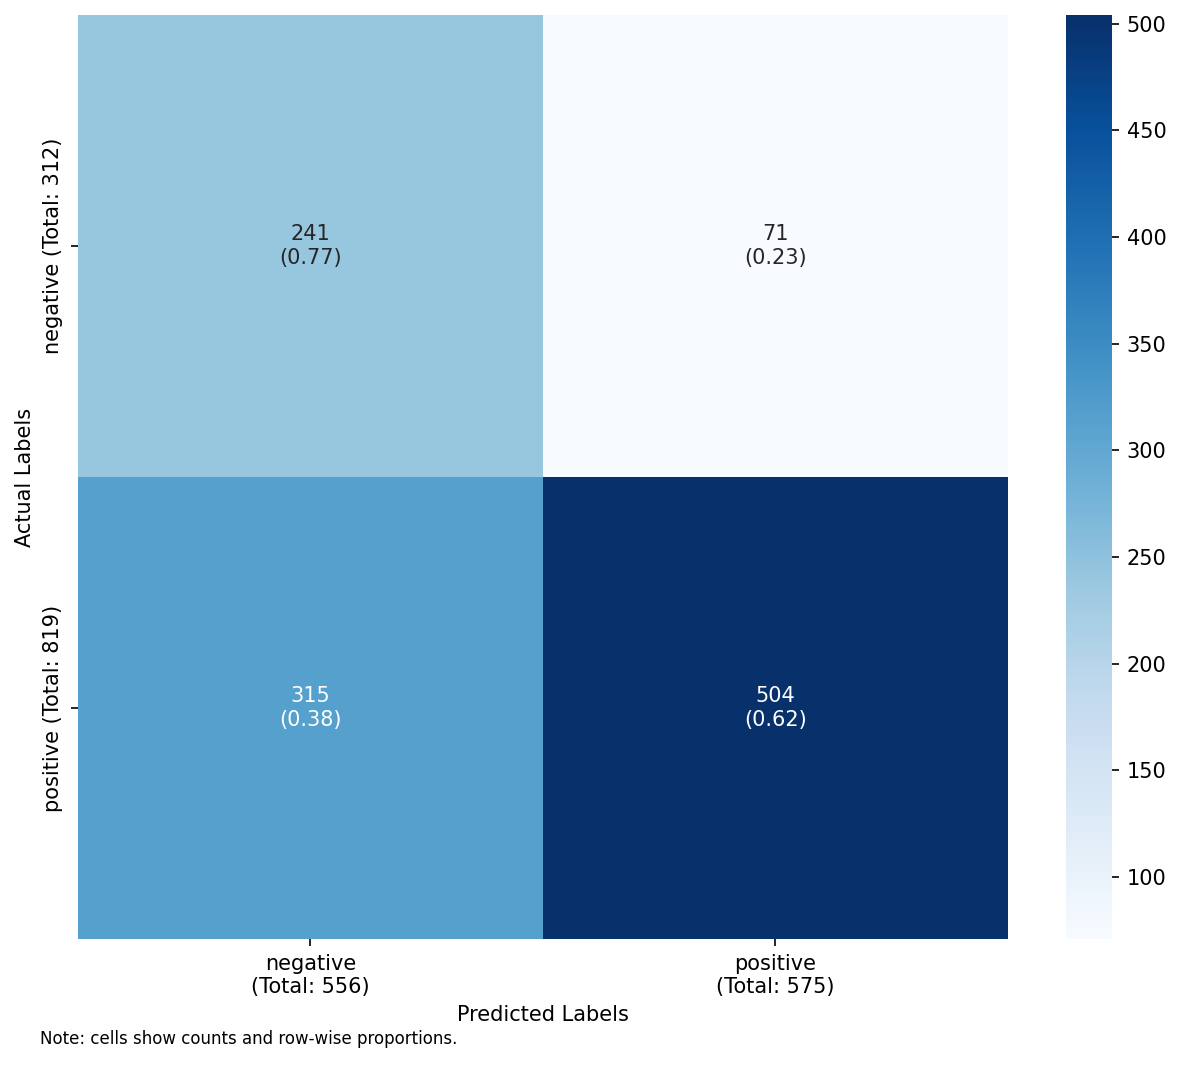
\includegraphics[width=0.48\textwidth]{media/cm_run3_lexicon_LR.png}
  \hfill
  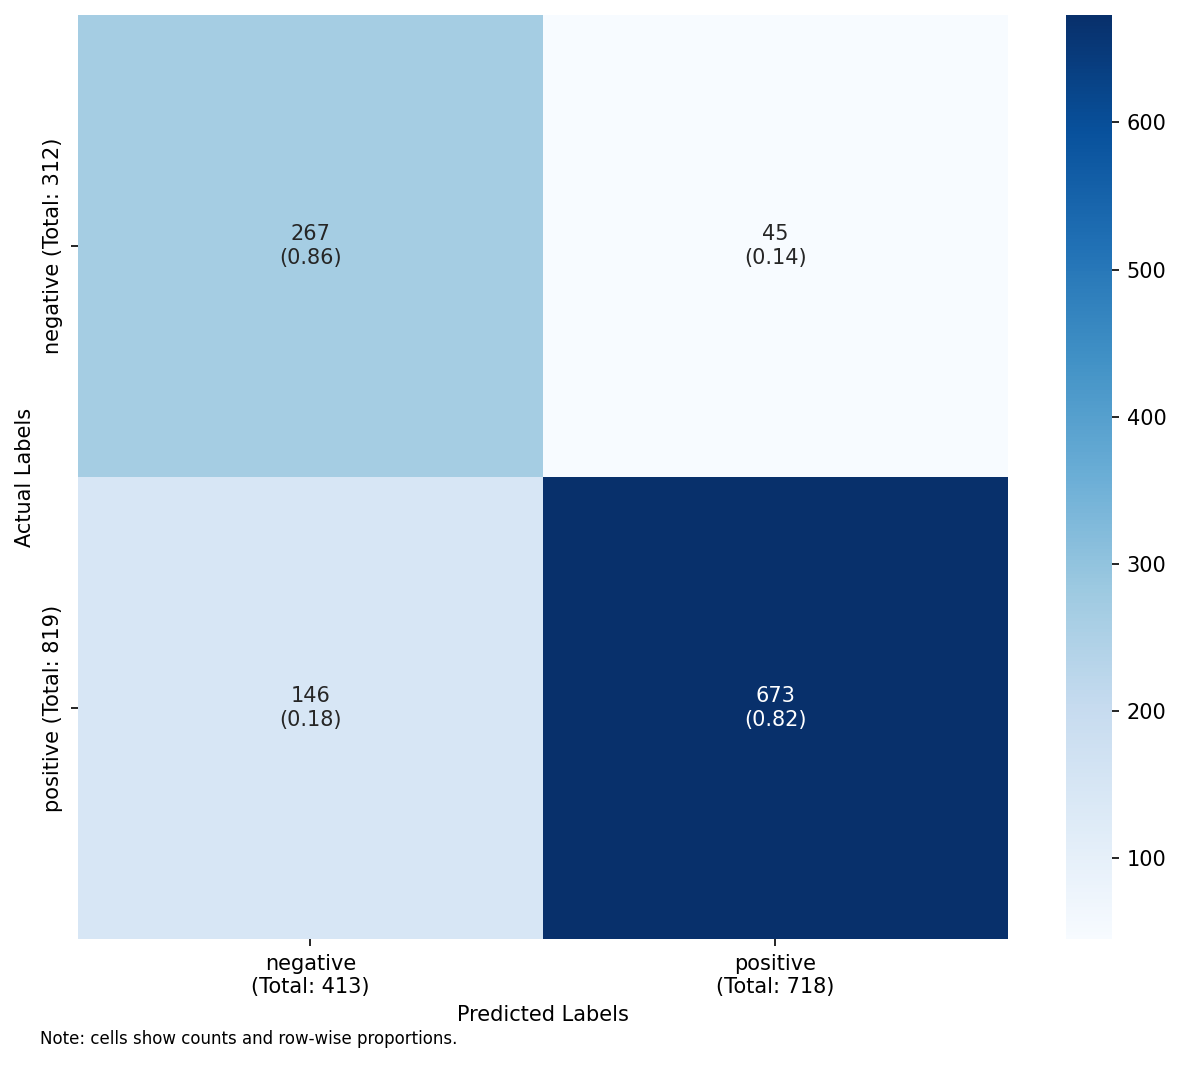
\includegraphics[width=0.48\textwidth]{media/cm_run3_embeddings_LR.png}
  \caption{RUN 3 LR: lexicon (left), embeddings (right)}
\end{figure}

\subsection*{RUN 4 --- binary, Decision Tree}

\begin{figure}[ht]
  \centering
  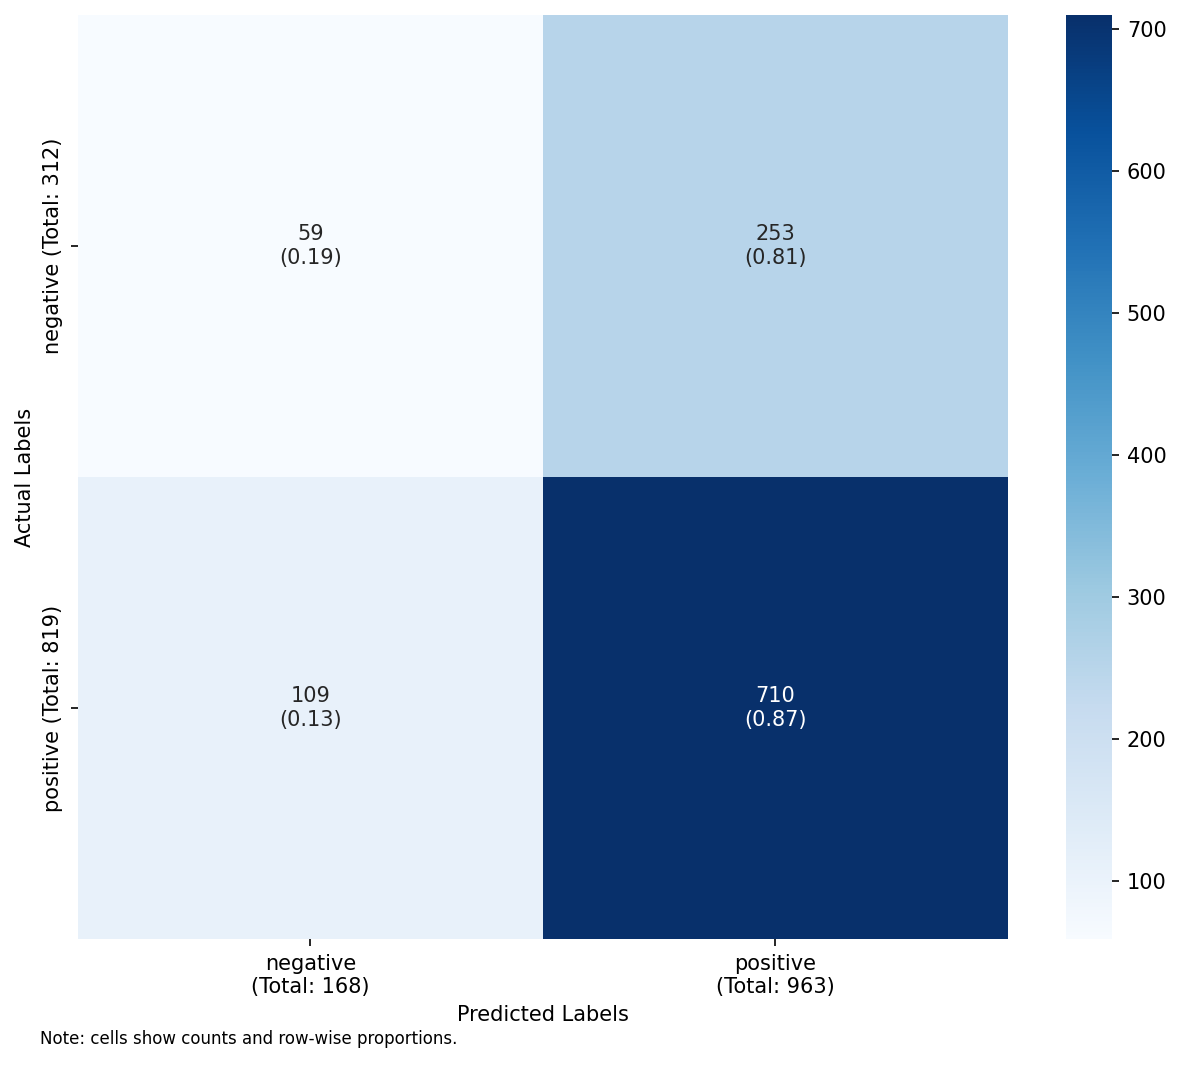
\includegraphics[width=0.48\textwidth]{media/cm_run4_unigrams_DT.png}
  \hfill
  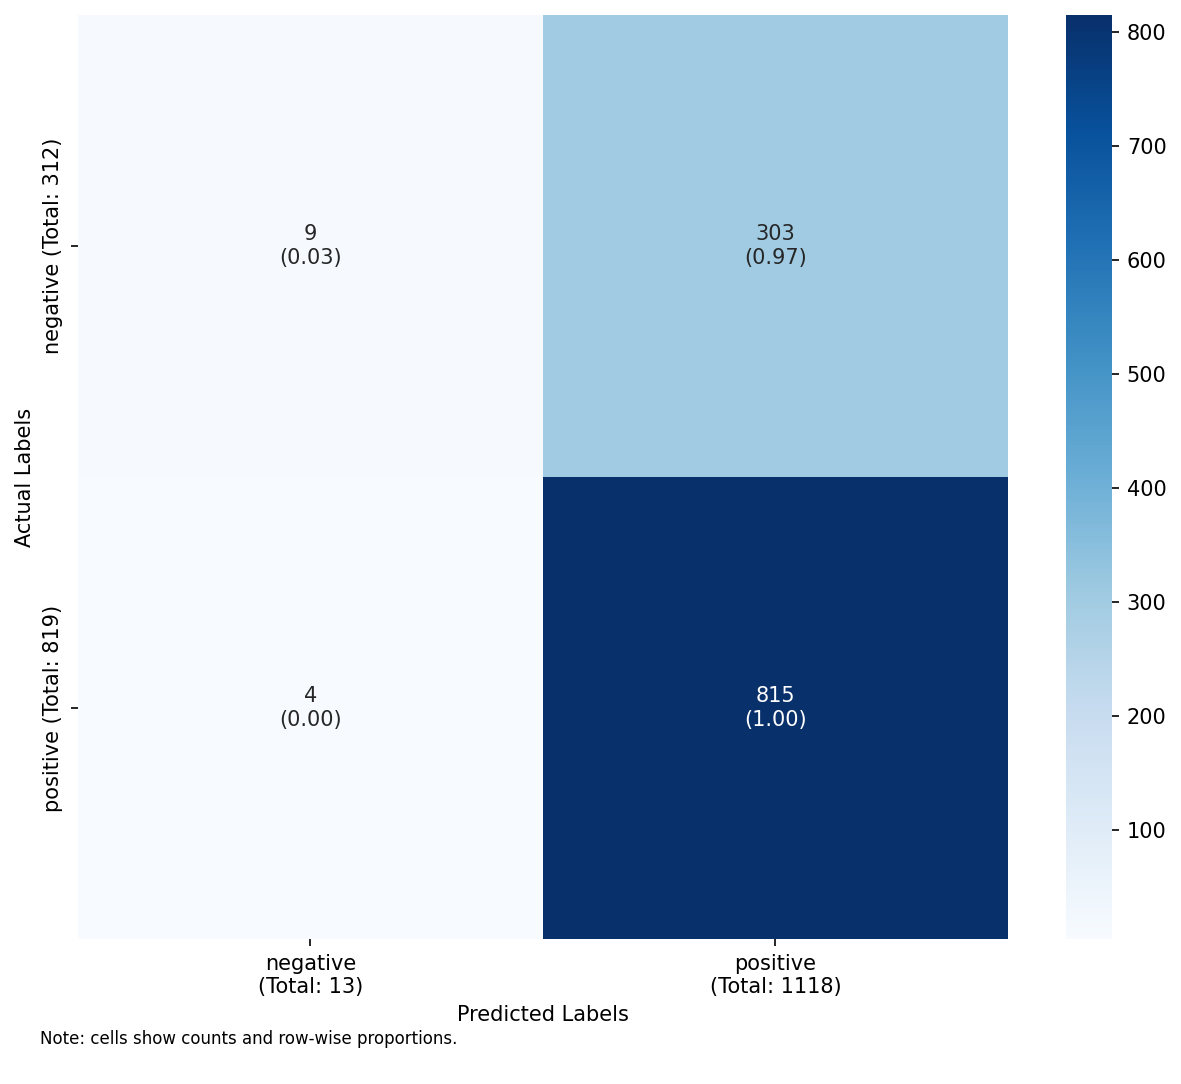
\includegraphics[width=0.48\textwidth]{media/cm_run4_bigrams_DT.png}
  \caption{RUN 4 DT: unigrams (left), bigrams (right)}
\end{figure}

\begin{figure}[ht]
  \centering
  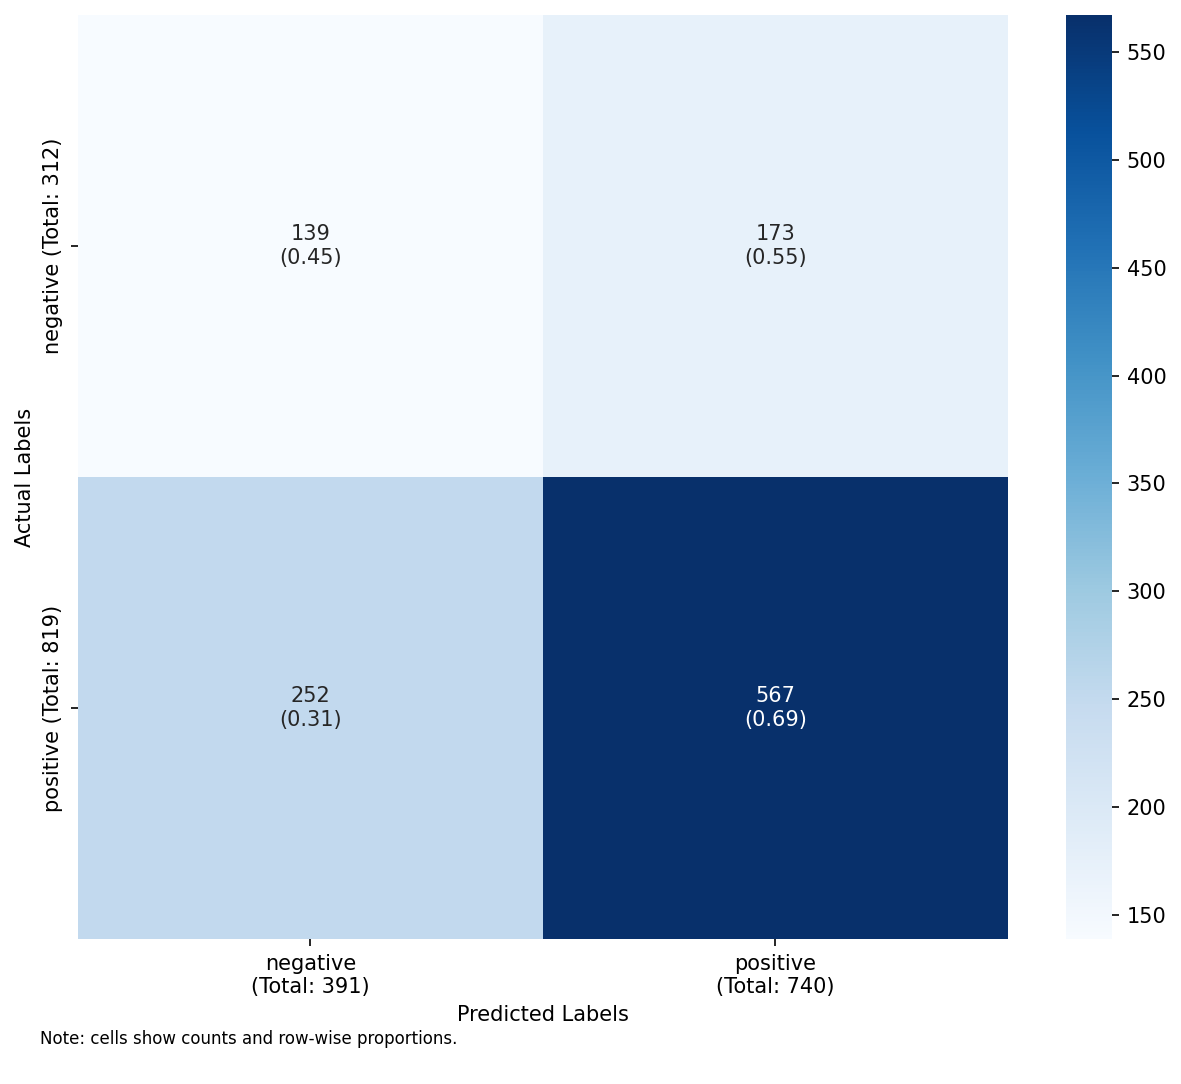
\includegraphics[width=0.48\textwidth]{media/cm_run4_uni+pos_DT.png}
  \hfill
  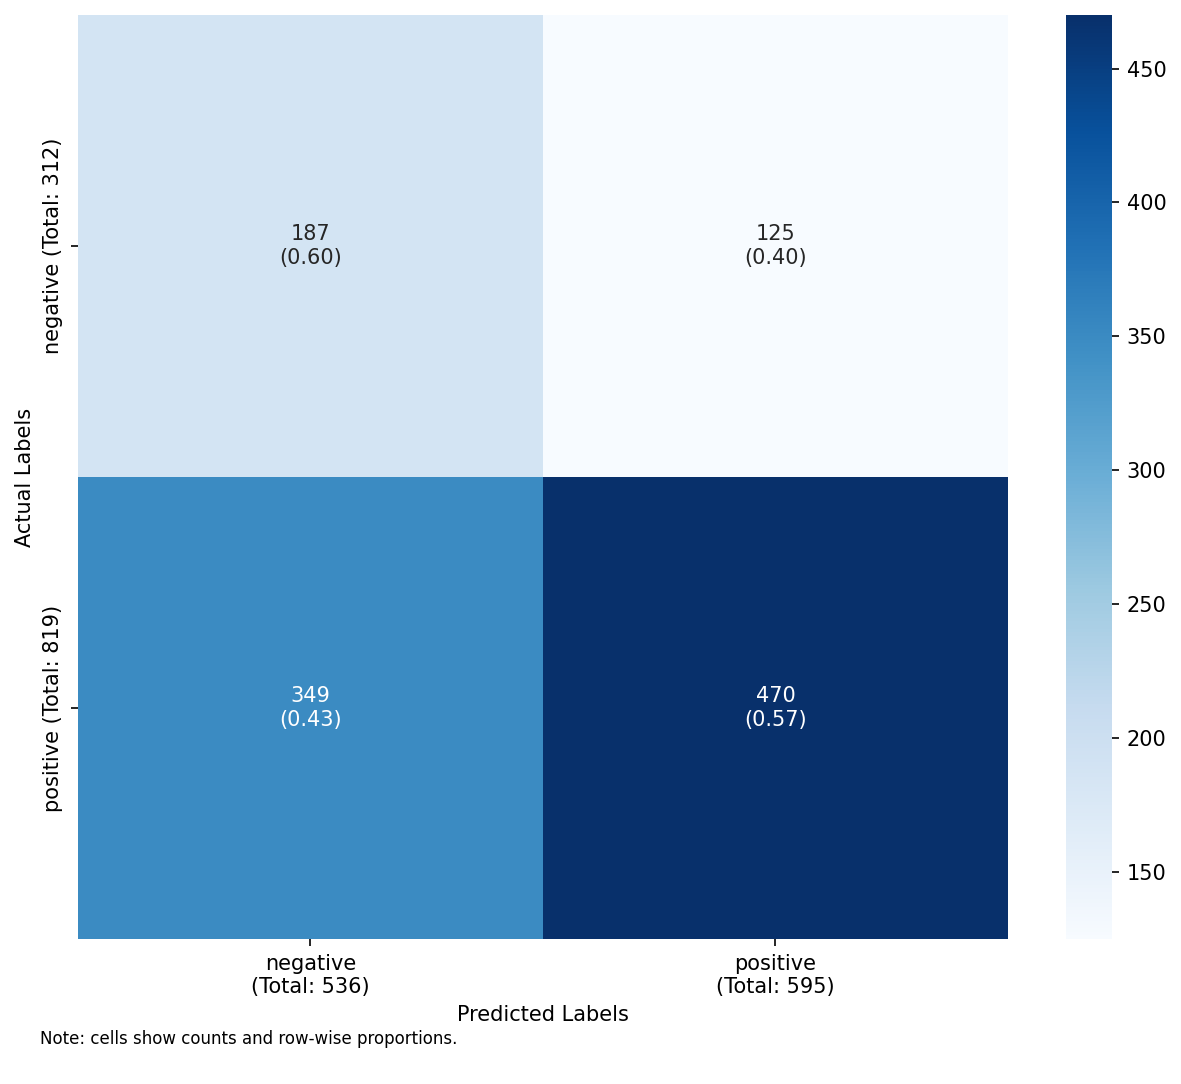
\includegraphics[width=0.48\textwidth]{media/cm_run4_textstats_DT.png}
  \caption{RUN 4 DT: unigrams+POS (left), text statistics (right)}
\end{figure}

\begin{figure}[ht]
  \centering
  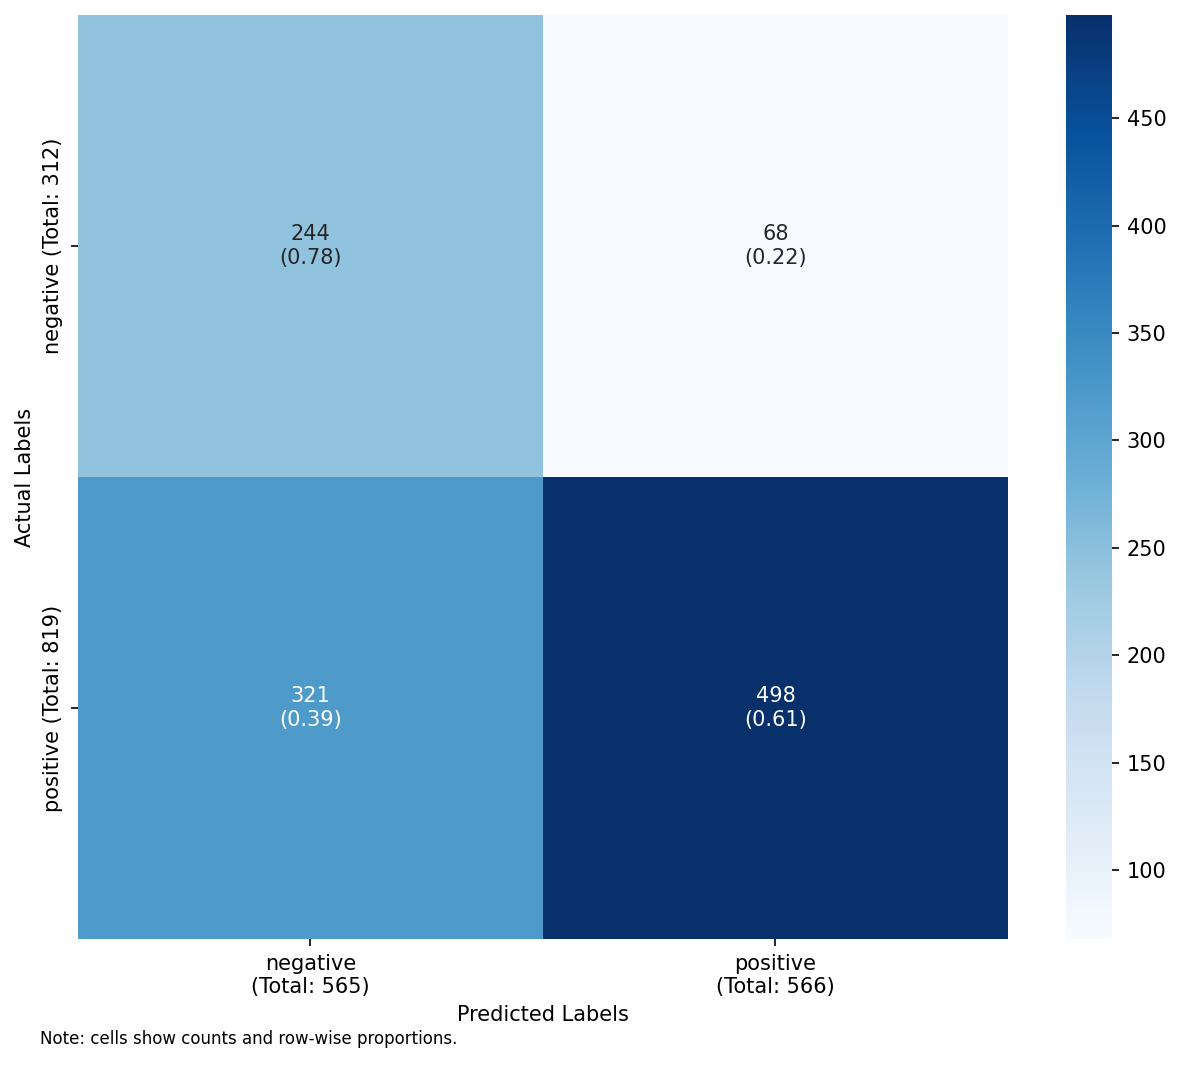
\includegraphics[width=0.48\textwidth]{media/cm_run4_lexicon_DT.png}
  \hfill
  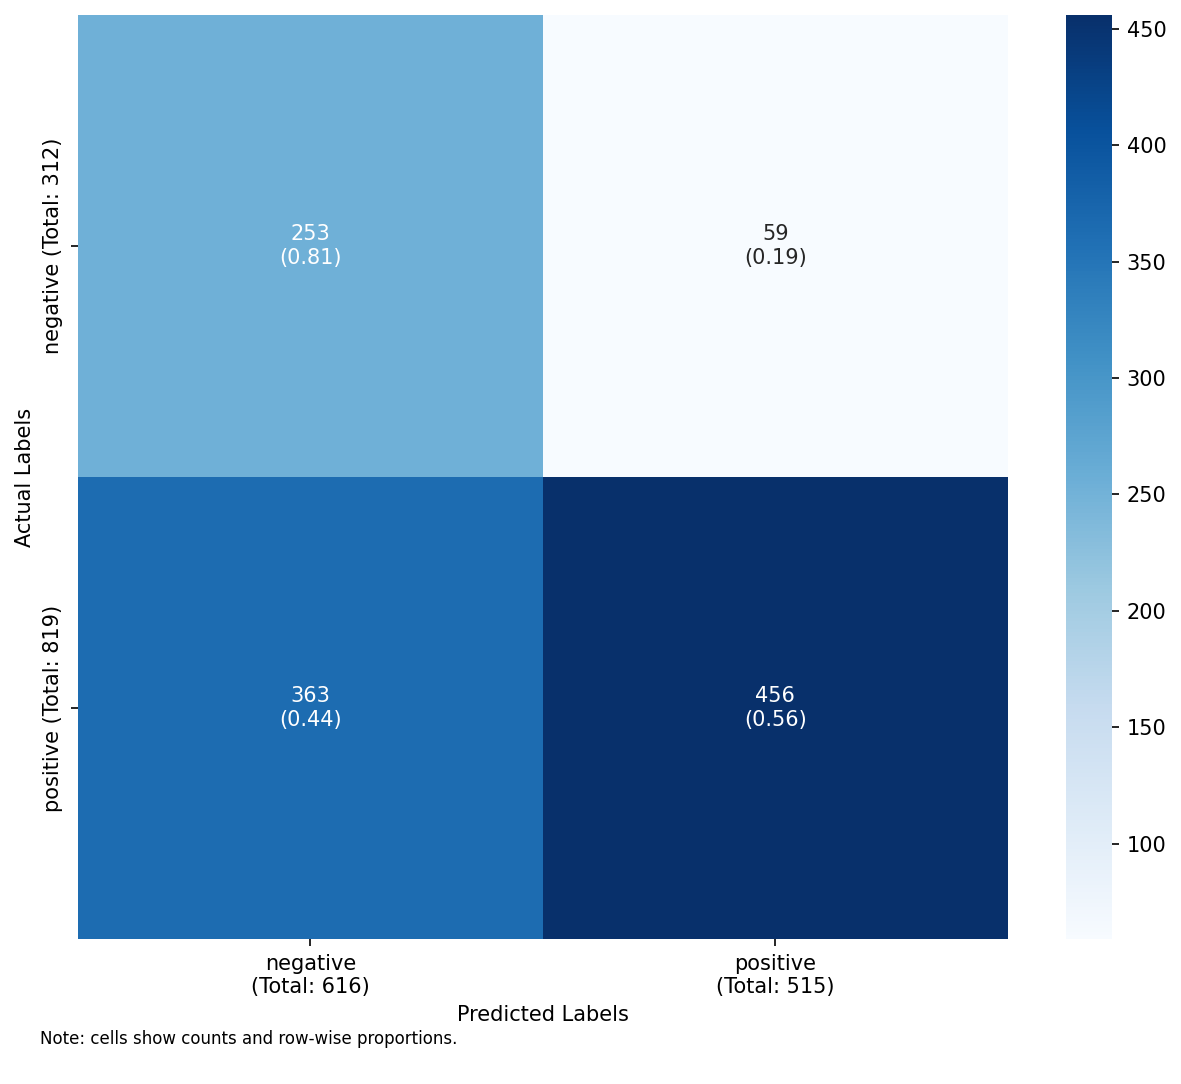
\includegraphics[width=0.48\textwidth]{media/cm_run4_embeddings_DT.png}
  \caption{RUN 4 DT: lexicon (left), embeddings (right)}
\end{figure}

\end{document}
